
\chapter{Applications of Multivariate Analysis in Metabolomics}

\section{Introduction}

\begin{doublespace}
This chapter details several varied applications of multivariate analysis
within the field of metabolomics, from the simplest examples of constructing
multivariate calibration models of \hnmr{} NMR spectral data for determination
of caffeine concentration in coffee, to more complex examples of multiblock
statistical modeling of joint \hnmr{} NMR and electrospray MS data. A final
note on the relationship between PCA scores-space class separations and OPLS-DA
model reliability is also presented to conclude the chapter.
\end{doublespace}

\section{\hnmr{} NMR Fingerprinting of Brewed Coffees}

\begin{doublespace}
To provide an initial illustration of the capabilities of the MVAPACK software
suite \cite{worley:acscb2014}, four roasts of brewed coffee were purchased from
a local coffee shop. In this study, \hnmr{} NMR and UV/Vis absorbance spectra
were collected in order to construct a multivariate calibration of \hnmr{} NMR
spectral information against caffeine concentration.
\end{doublespace}

\subsection{Materials and Methods}

\subsubsection{Coffee Sample Preparation}

\begin{doublespace}
Four freshly brewed roasts of coffee (Light, Dark, Medium Regular and Medium
Decaffeinated) were purchased from a local coffee shop. From each roast,
sixteen 1.2 mL samples were drawn while the coffee was still hot and stored
at $-80^\circ$C for 24 hours. The samples were then lyophilized at
$-50^\circ$C and 0.1 mBar for 24 hours and subsequently redissolved in 1.0 mL
of 99.8\% D$_2$O (Isotec, St. Louis, MO) without pH adjustment. Following
redissolution, the samples were centrifuged at 12,000 RPM and $25^\circ$C
for 5 minutes and 800 $\mu$L of the supernatant was collected into NMR tubes.
The samples were stored in their NMR tubes at $4^\circ$C for 36 hours prior
to data collection.
\end{doublespace}

\subsubsection{Caffeine Extraction}

\begin{doublespace}
Measurement of the caffeine concentration in each coffee roast was performed
based on previously outlined procedures \cite{belay:food2008}. Triplicate
standards of caffeine were made by dissolving 2.9 mg of caffeine
(Sigma-Aldrich, St. Louis, MO) into 100.0 mL of 99.5\% CH$_2$Cl$_2$
(Sigma-Aldrich, St. Louis, MO) for a final concentration of 149 $\mu$M.
From each purchased coffee roast, 25 mL of brewed coffee were combined with
25 mL of CH$_2$Cl$_2$ in a separatory funnel in a two-step liquid-liquid
extraction. Extracted caffeine in CH$_2$Cl$_2$ was diluted 20-fold into 1.0
mL and subjected to UV/Vis absorption spectroscopy for caffeine quantitation.
\end{doublespace}

\begin{figure}[ht!]
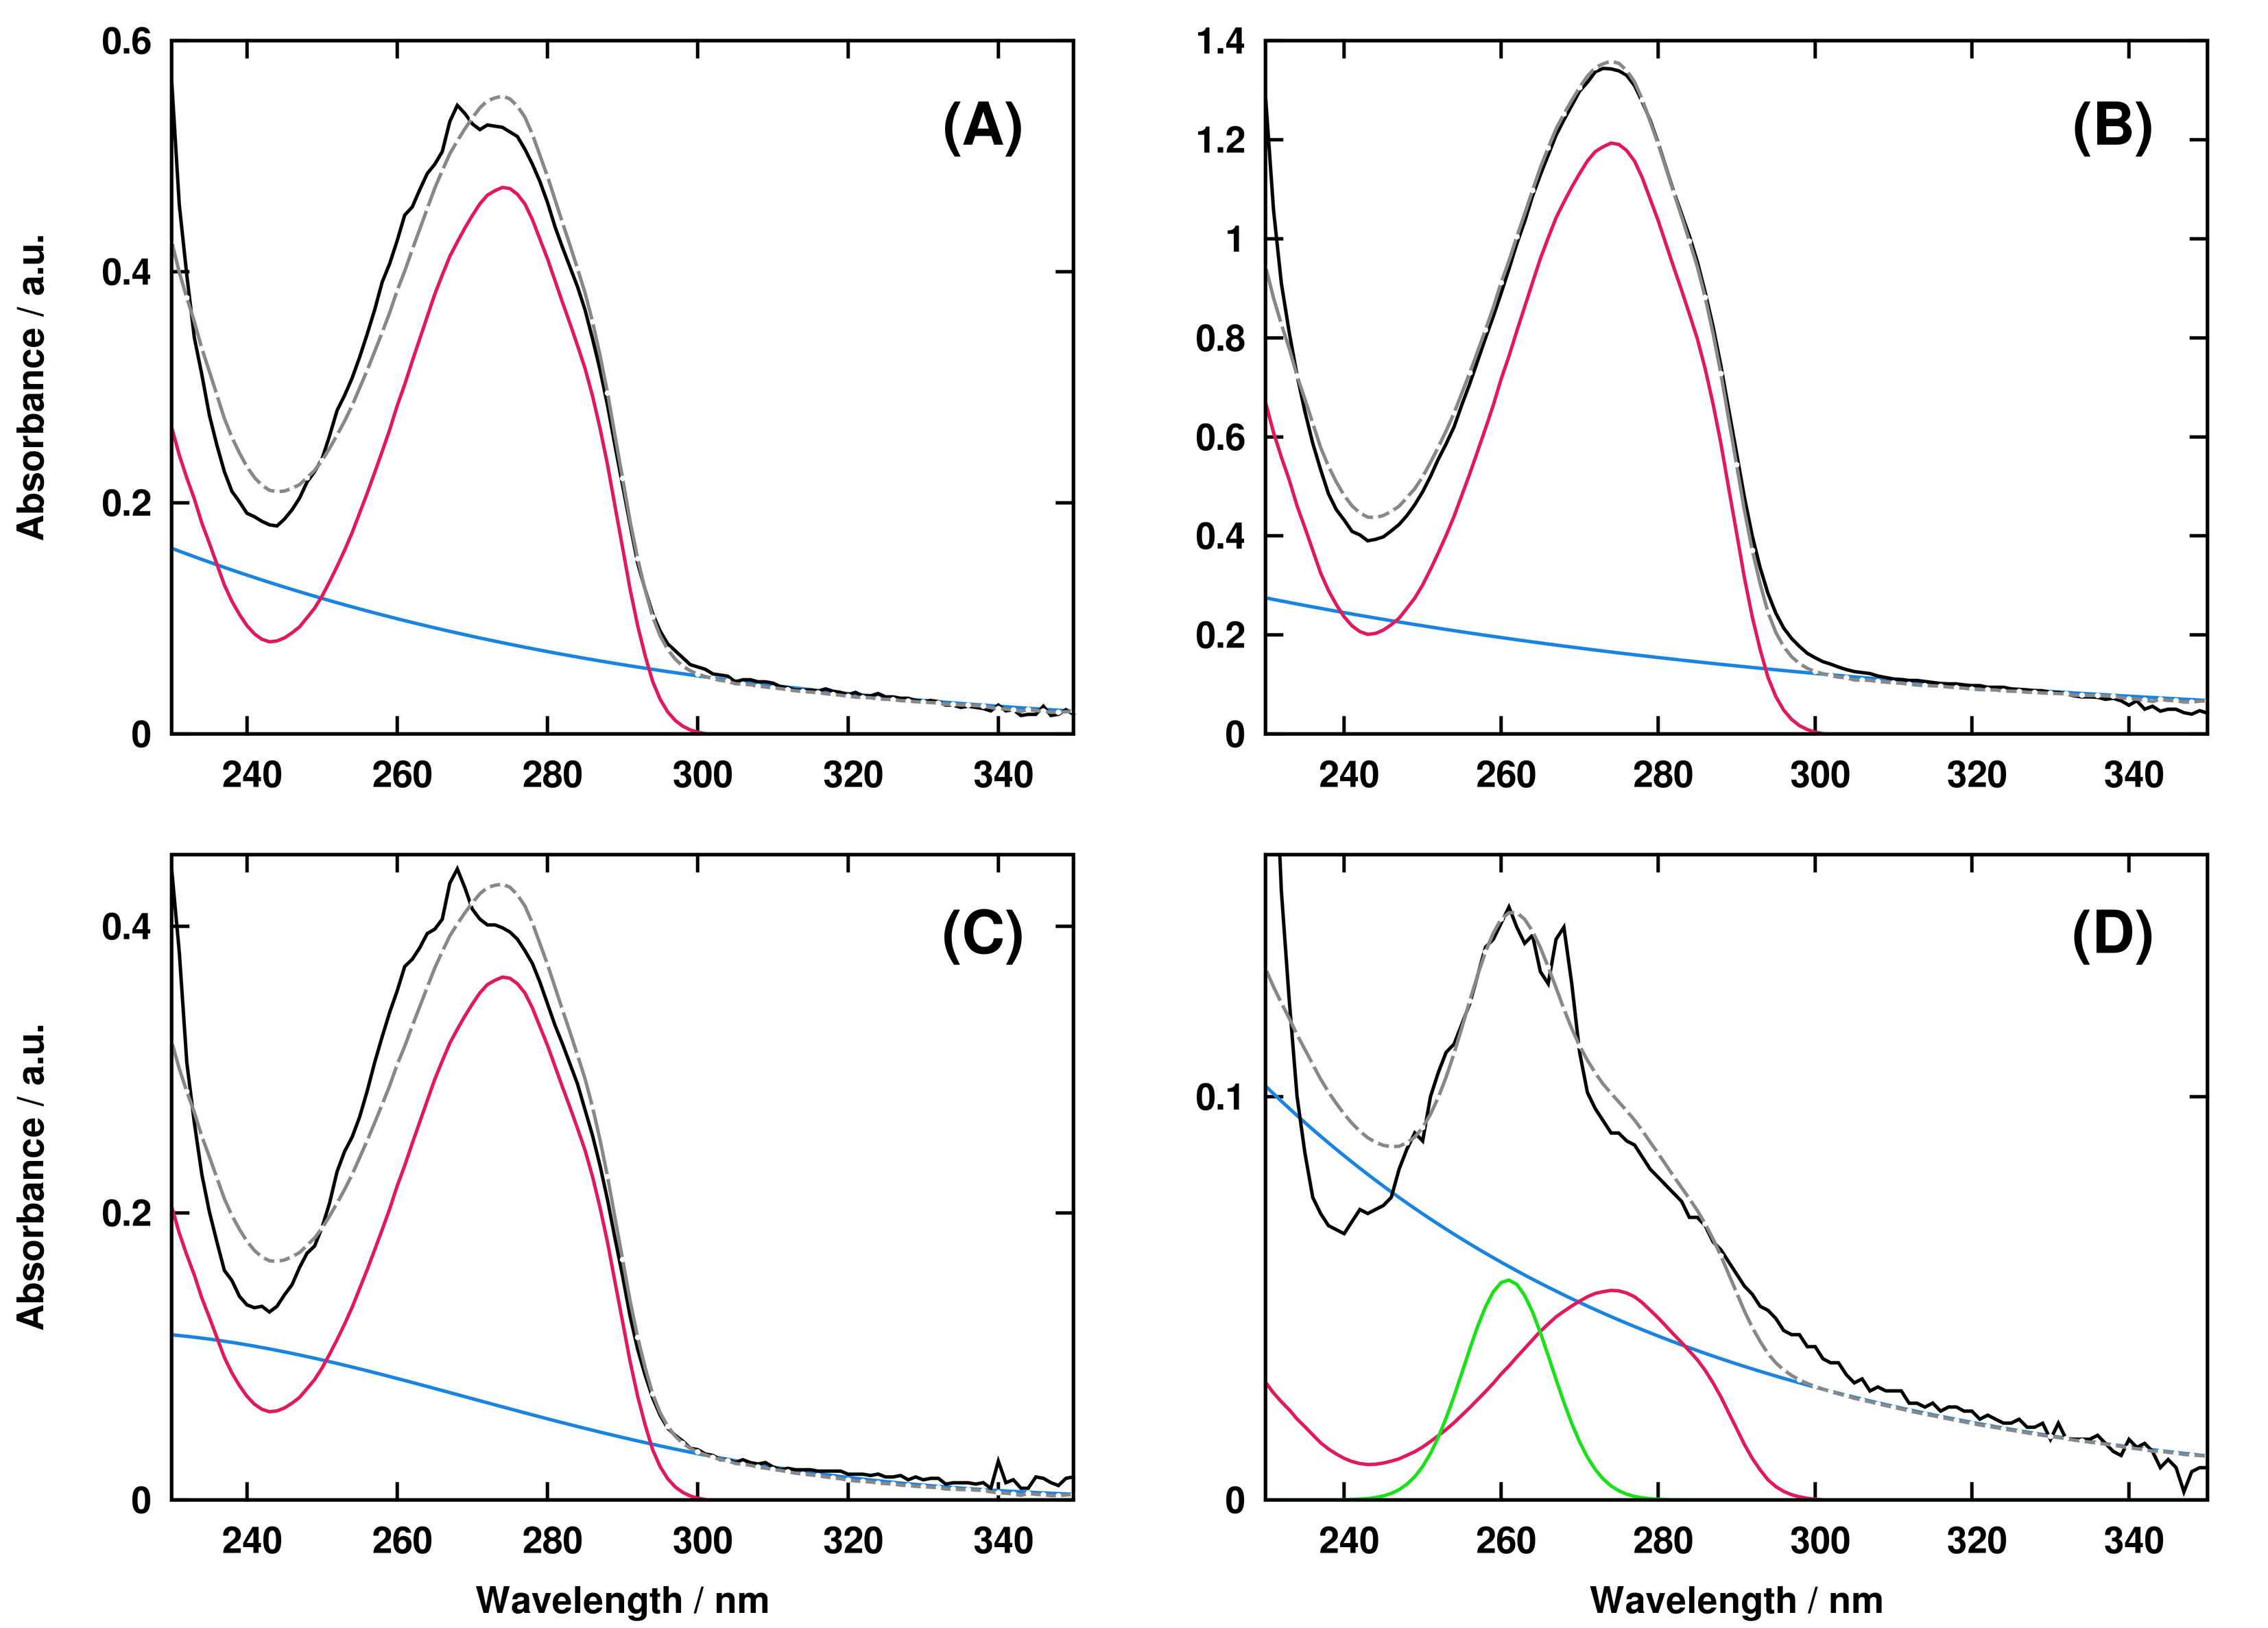
\includegraphics[width=6.5in]{figs/apps/01-uvfit.png}
\caption
      [UV/Vis Caffeine Quantitation Band-fitting Results.]{
  {\bf UV/Vis Caffeine Quantitation Band-fitting Results.}
  \\
  UV/Vis absorbance band-fitting results for caffeine concentration estimation
  of dark roast ({\bf A}), light roast ({\bf B}), regular medium roast
  ({\bf C}), and decaffeinated medium roast ({\bf D}). Black lines represent
  observed spectra, dashed grey lines represent fitted spctra, red lines
  represent fitted caffeine, and blue and green lines represent additional
  Gaussian bands required for fitting.
}
\end{figure}

\subsubsection{UV/Vis Spectroscopy}

\begin{doublespace}
Absorption spectra of caffeine standards and extracts were collected on a
Shimadzu UV-2501PC with a 1.0 nm slit width and 1.0 cm quartz cuvettes. Spectra
were collected between the wavelengths of 500 nm and 230 nm.
\end{doublespace}

\subsubsection{NMR Spectroscopy}

\begin{doublespace}
All NMR experiments were collected on a Bruker Avance DRX 500 MHz spectrometer
equipped with a 5 mm inverse triple-resonance (\hnmr{}, \cnmr{}, \nnmr{})
cryoprobe with a $z$-axis gradient. A Bruker BACS-120 sample changer and
ICON-NMR software were used to automate NMR data collection. A standard 1D
\hnmr{} NMR spectrum using a SOGGY pulse sequence
\cite{hwang:jmr1995,nguyen:jmr2007} and a $T_2$-filtered 1D \hnmr{} NMR
spectrum using a $z$-filtered Carr-Purcell-Meiboom-Gill (CPMG) sequence
\cite{rastrelli:jacs2009} with an identical SOGGY water suppression element
were acquired for each sample. All experiments were performed at $20^\circ$C
with 128 scans, 32 dummy scans, a carrier frequency offset of 2,351 Hz, a
6,009 Hz spectral width, and a 1.0 s inter-scan delay. For $T_2$ filtered
spectra, 20 repetitions of a CPMG-$z$ element having a delay ($\tau$) of 5.0
ms were performed per scan, for a total filter time ($2n\tau$) of 200.0 ms.
Free induction decays were collected with 32,768 total data points resulting
in a total acquisition time of 10 minutes per experiment.
\end{doublespace}

\subsubsection{Caffeine Quantitation}

\begin{doublespace}
A reference spectrum of caffeine in CH$_2$Cl$_2$ was generated from the three
standard UV/Vis absorption spectra by taking the mean of the spectra after
multiplicative scatter correction (MSC, \cite{fearn:cils2009}). To quantify
caffeine in the extracts, the absorption spectrum of each extract was fit by
nonlinear least squares \cite{marquardt:jsiam1963} to the sum of the scaled
caffeine reference spectrum and no more than two extra `background' Gaussian
bands (Figure 4.1). The ratio of the fit caffeine reference spectrum in each
extract to that of the known samples was used as an estimate of caffeine
concentration in the extracts. Concentrations of the medium regular, medium
decaffeinated, dark and light roasts were 1.526 mM, 0.217 mM, 1.979 mM and
4.993 mM, respectively.
\end{doublespace}

\subsubsection{Multivariate Analysis}

\begin{doublespace}
All NMR spectra were loaded, processed, treated and modeled inside the GNU
Octave 3.6 programming environment \cite{eaton2008} using functions available
in the MVAPACK software suite for chemometrics \cite{worley:acscb2014}.
Free induction decays were loaded in from Bruker DMX binary format and
corrected for group delay errors by a circular shift of their time-domain
data points. All decays were Fourier transformed, automatically phase-corrected
and referenced to match the chemical shifts of caffeine with known database
values. Spectral regions upfield of 0.44 ppm and downfield of 9.16 ppm were
removed from the dataset, as they contained no informative signals. As solvent
resonances were adequately suppressed by the excitation sculpting pulse
sequence, no spectral regions were removed around the water resonance.
Figure 4.2 illustrates the final result of spectral processing of the coffees
dataset using MVAPACK.
\end{doublespace}

\begin{figure}[ht!]
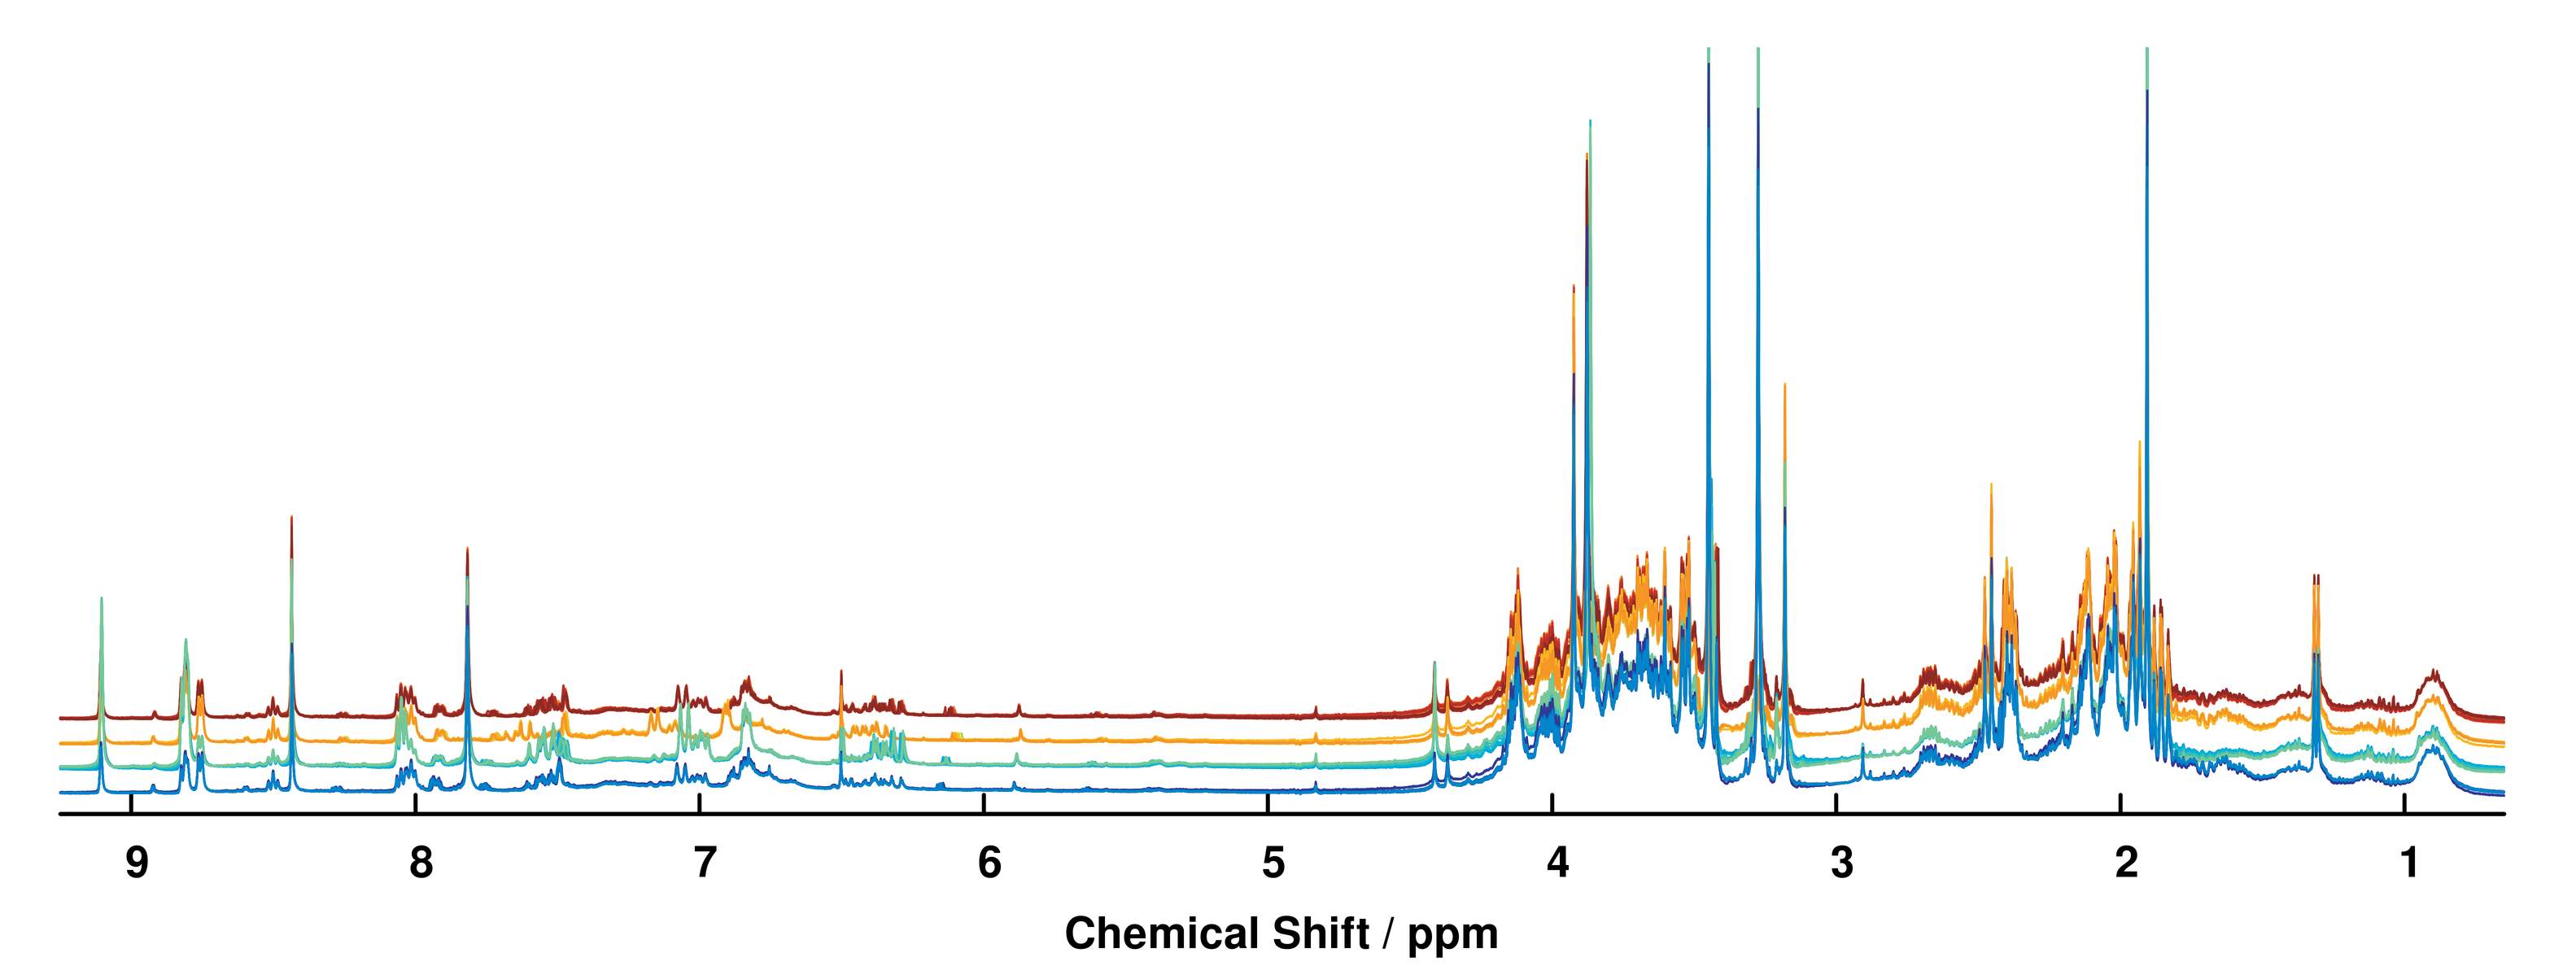
\includegraphics[width=6.5in]{figs/apps/02-spectra.png}
\caption
      [Processed \hnmr{} NMR Spectra of Coffee Roasts.]{
  {\bf Processed \hnmr{} NMR Spectra of Coffee Roasts.}
  \\
  Representative processed 1D \hnmr{} NMR spectra for all spectra of each
  coffee roast, acquired using the water-suppressed CPMG-$z$ pulse sequence
  and processed in MVAPACK. To reach this point, free induction decays were
  simply Fourier transformed and automatically phased. No manual phase
  corrections were applied after autophasing.
}
\end{figure}

\begin{doublespace}
For principal component analysis (PCA), the dataset was normalized by the
method of probabilistic quotients (PQ, \cite{dieterle:anchem2006}) and
subjected to adaptive intelligent binning \cite{demeyer:anchem2008}.
Low-variation `noise' bins were automatically removed from the dataset
\cite{zhang:opin2008}, resulting in a final data matrix having 64 observations
and 284 variables. The data matrix was scaled to unit variance
\cite{vandenberg:bmcg2006} prior to NIPALS PCA modeling \cite{jolliffe2002},
which produced six significant components having cumulative \rsqx{} and
\qsq{} statistics of 0.9689 and $0.8965 \pm 0.0105$, respectively
\cite{eshghi:cils2014}.
\\\\
Linear discriminant analysis (LDA) was performed on the first three dimensions
of resulting PCA scores to yield a two-component model that best
captured the between-class variation present in the three orthonormal PCA
score vectors. LDA modeling yielded a model having a cumulative \rsqx{}
statistic of 0.9950 and cumulative \rsqy{} and \qsq{} statistics of 1.0.
Scores from the PCA model of the coffees \hnmr{} NMR spectral data, and
their corresponding LDA projection, are shown in Figure 4.3.
\end{doublespace}

\begin{figure}[ht!]
\includegraphics[width=6.5in]{figs/apps/03-pca-lda.png}
\caption
      [Principal Component Scores of the Coffees Spectra.]{
  {\bf Principal Component Scores of the Coffees Spectra.}
  \\
  PCA ({\bf A}) and LDA ({\bf B}) scores of the four coffee roasts. Red,
  green, blue and violet points represent dark, light, decaffeinated medium,
  and regular medium roasts, respectively. Ellipsoids and ellipses enclose
  the 95\% confidence intervals estimated by the sample means and covariances
  of scores from each class. Axis labels in panels ({\bf A}) and ({\bf B})
  indicate scores in PCA and LDA bases, respectively, and not the same set
  of scores.
}
\end{figure}

\begin{doublespace}
For orthogonal projections to latent structures regression
(OPLS-R, \cite{trygg:jchemo2002}), the full-resolution dataset was aligned
using a per-class application of interval correlation-optimized shifting
(\emph{i}COshift, \cite{savorani:jmr2010}) and PQ normalization, resulting
in a final data matrix having 64 observations and 11,888 variables. The
Pareto-scaled data matrix was regressed by OPLS against a response vector
containing caffeine concentrations estimated by UV/Vis analysis of the four
coffee roasts, yielding a model with one predictive component and one
orthogonal component (\rsqxp{} = 0.5294, \rsqxo{} = 0.1288, \rsqy{} = 0.9822,
\qsq{} = $0.9502 \pm 0.0008$). CV-ANOVA significance testing returned a $p$
value equal to zero ($F$ = 2258.8) to within double-precision floating point
error, indicating a reliable model. The OPLS-R and LDA models were further
validated using response permutation tests having 1,000 iterations each. The
permutation tests of both models resulted in $p$ values less than 0.001 for
both \rsqy{} and \qsq{}, a further indication of high model reliability.
\end{doublespace}

\subsubsection{Validation against SIMCA-P+}

\begin{doublespace}
Correctness of the PCA and OPLS-R models generated by MVAPACK was verified by
exporting the final processed and treated data matrices from GNU Octave and
modeling them in SIMCA-P+ 13.0 (Umetrics AB, Umea, Sweden). The scores
extracted from SIMCA and MVAPACK were found to have coefficients of
determination (\rsq{}) of 0.999976 and 0.999989 for the PCA and OPLS models,
respectively. The `imperfect' non-unity values of \rsq{} reflect the fact that
SIMCA-P+ 13.0 only permits the export of scores with no more than four decimal
places.
\end{doublespace}

\begin{SCfigure}
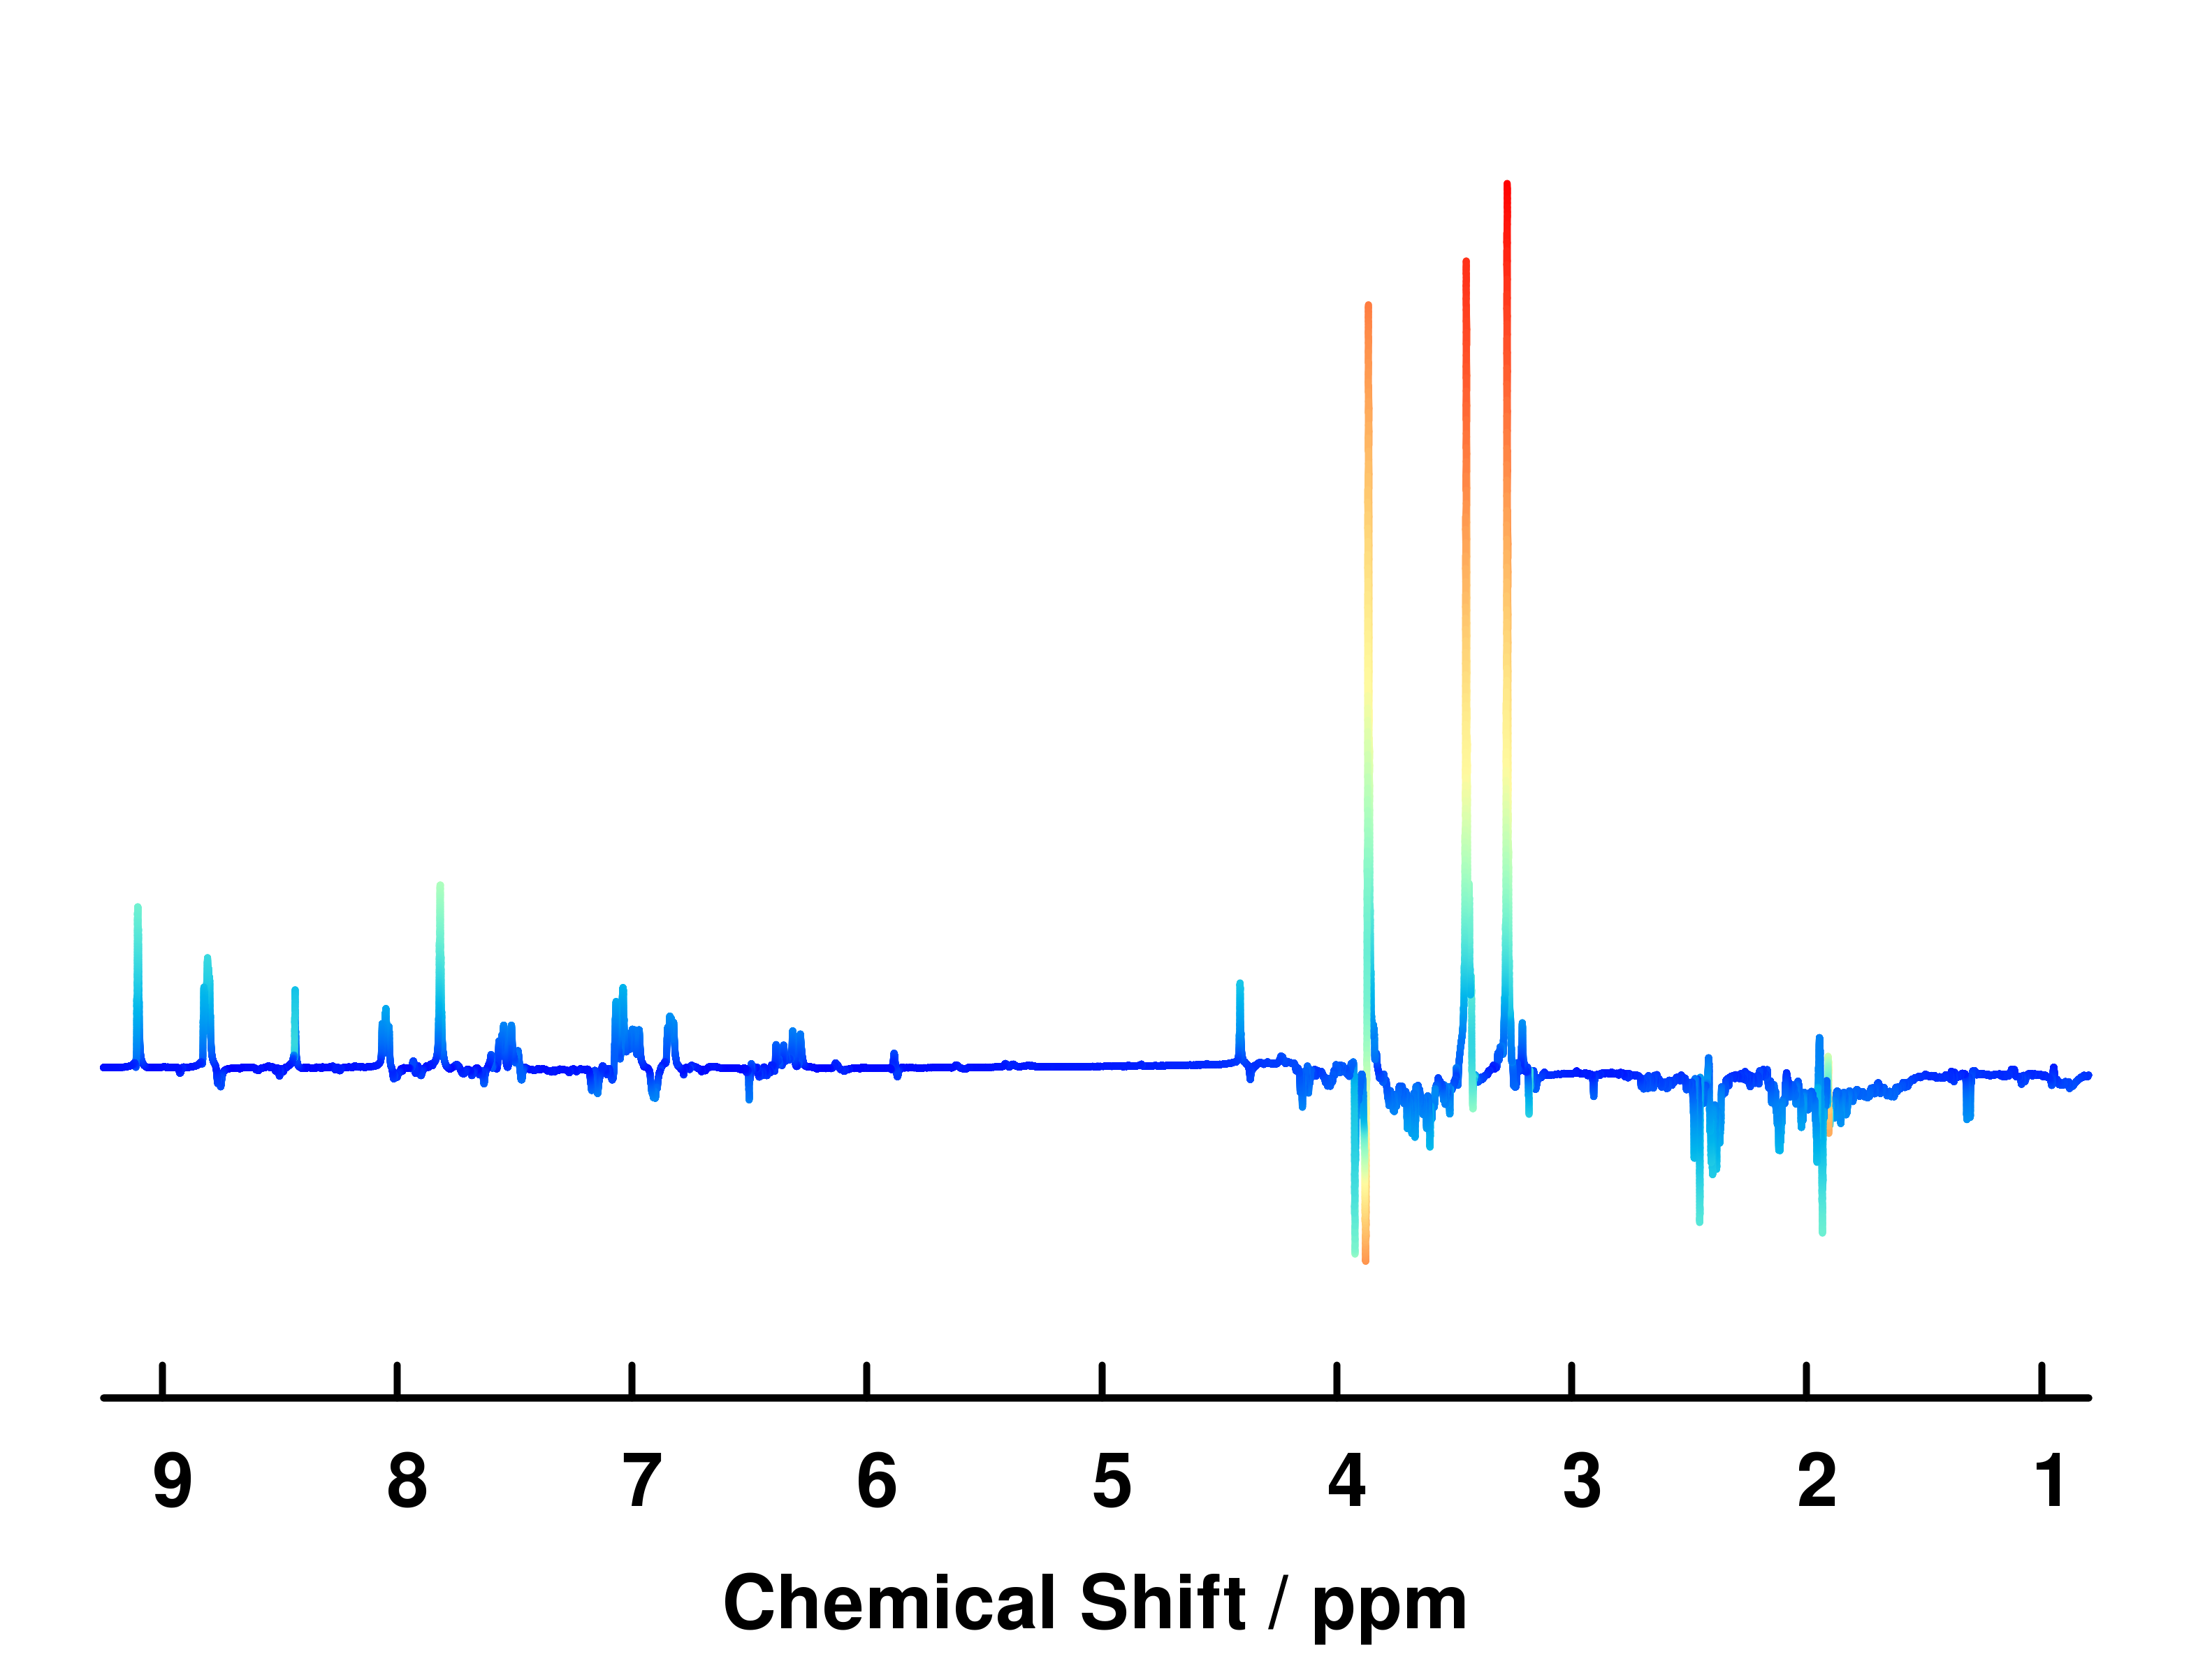
\includegraphics[width=3.5in]{figs/apps/04-oplsr-p.png}
\caption
      [Backscaled Coffees OPLS-R Model Loadings.]{
  {\bf Backscaled Coffees OPLS-R Model Loadings.}
  \\
  Backscaled OPLS-R predictive loadings of the four coffee roasts regressed
  according to estimated caffeine concentration. The pseudospectral nature of
  backscaled loadings facilitates analysis of model results by any
  spectroscopist. The four most intense positive positive peaks in the
  loadings pseudospectrum correspond directly to caffeine NMR resonances
  archived in the BMRB, indicating a fairly successful regression against
  caffeine concentration.
}
\end{SCfigure}

\subsection{Results and Discussion}

\begin{doublespace}
Use of MVAPACK during analysis of the coffees dataset arguably facilitated
rapid identification of ideal processing, treatment and modeling parameters
during data handling. Use of automatic phase correction, adaptive intelligent
binning, and PQ normalization yielded a dataset in which three principal
components were sufficient to fully separate all classes in scores space,
and subsequent LDA modeling resulted in complete class separation in only
two components (Figure 4.3).
\\\\
As opposed to the PCA modeling procedure, which utilized binned spectra,
OPLS-R model training was performed using full-resolution 1D \hnmr{} NMR
spectra in order to reap the interpretive advantages of full-resolution
backscaled loadings (Figure 4.4). The availability of \emph{i}COshift
alignment \cite{savorani:jmr2010} in MVAPACK effectively makes the modeling
of full-resolution NMR spectral data possible by correcting positional noise
\cite{aberg:abc2009} in the spectra that corrupts the bilinear nature of the
data. By regressing the NMR data against estimates of caffeine concentration
obtained by UV/Vis spectroscopy (Figure 4.1), a loading pseudo-spectrum of
caffeine was obtained that matched almost perfectly with spectral data
deposited in the Biological Magnetic Resonance Bank \cite{ulrich:nar2008}.
It is conceivable that spectral features coextracted with caffeine in the
loadings correspond to coffee bean metabolites lost alongside caffeine during
roasting or decaffeination.
\end{doublespace}

\begin{figure}[H]
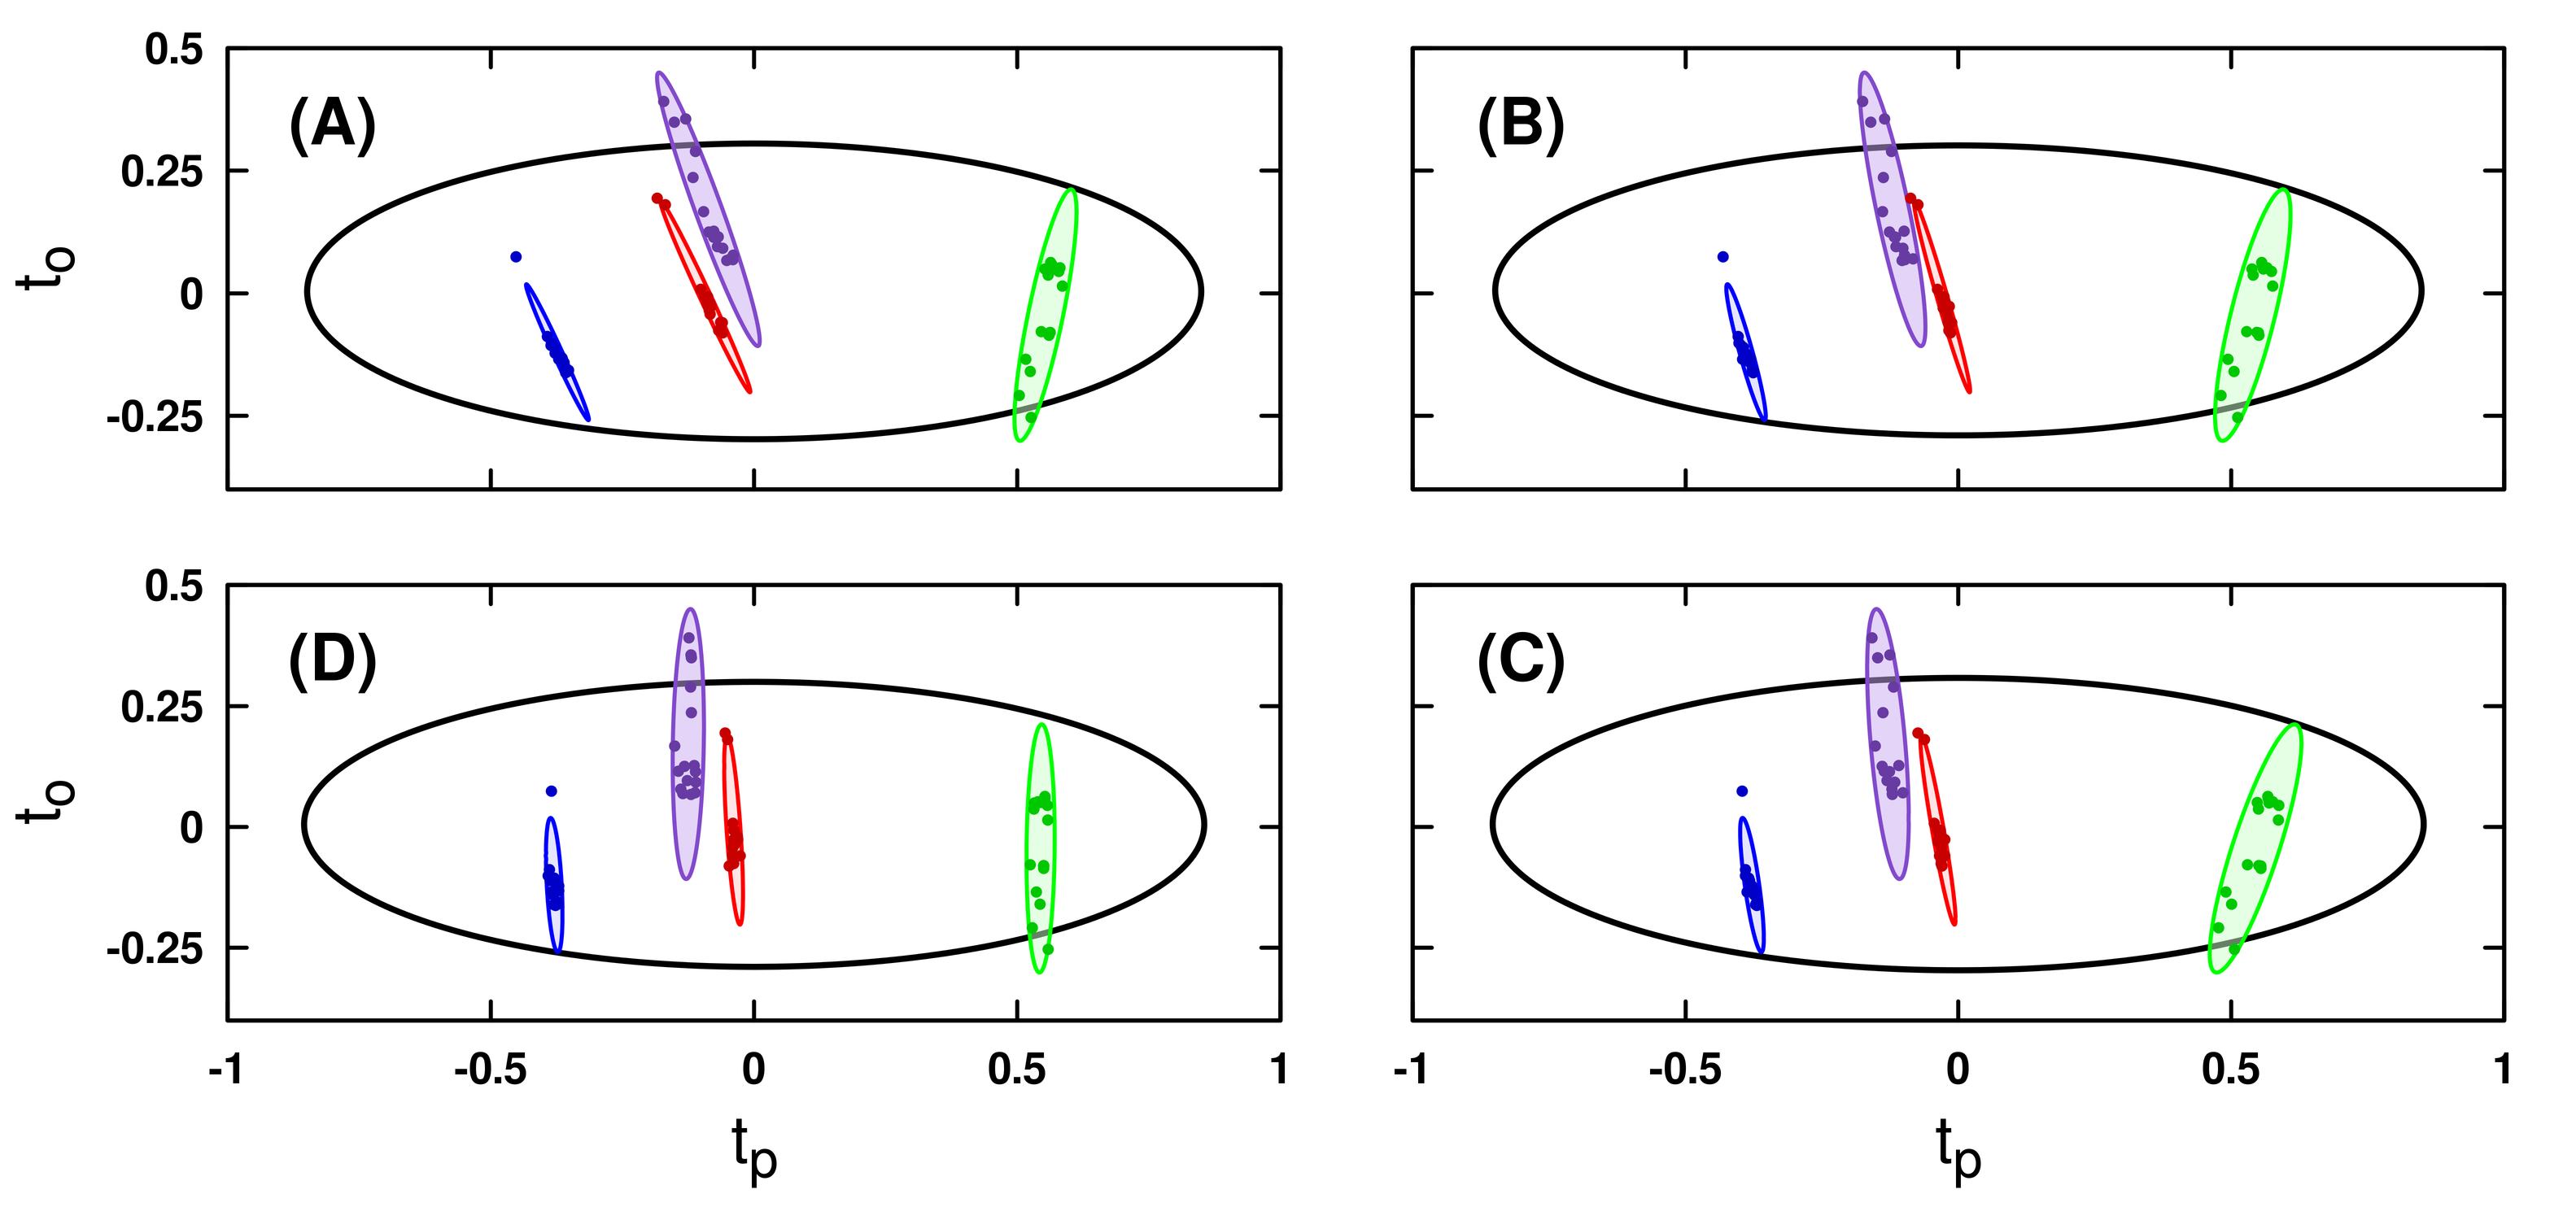
\includegraphics[width=6.5in]{figs/apps/05-oplsr-t.png}
\caption
      [Coffees OPLS-R Scores as Evidence of Overfit.]{
  {\bf Coffees OPLS-R Scores as Evidence of Overfit.}
  \\
  OPLS-R scores of the four coffee roasts, where each roast was regressed
  against its caffeine concentration estimated by UV/Vis absorbance
  spectroscopy. Scores in panels ({\bf A}) through ({\bf D}) were computed
  from models having 1 through 4 orthogonal components, respectively.
}
\end{figure}

\begin{figure}[H]
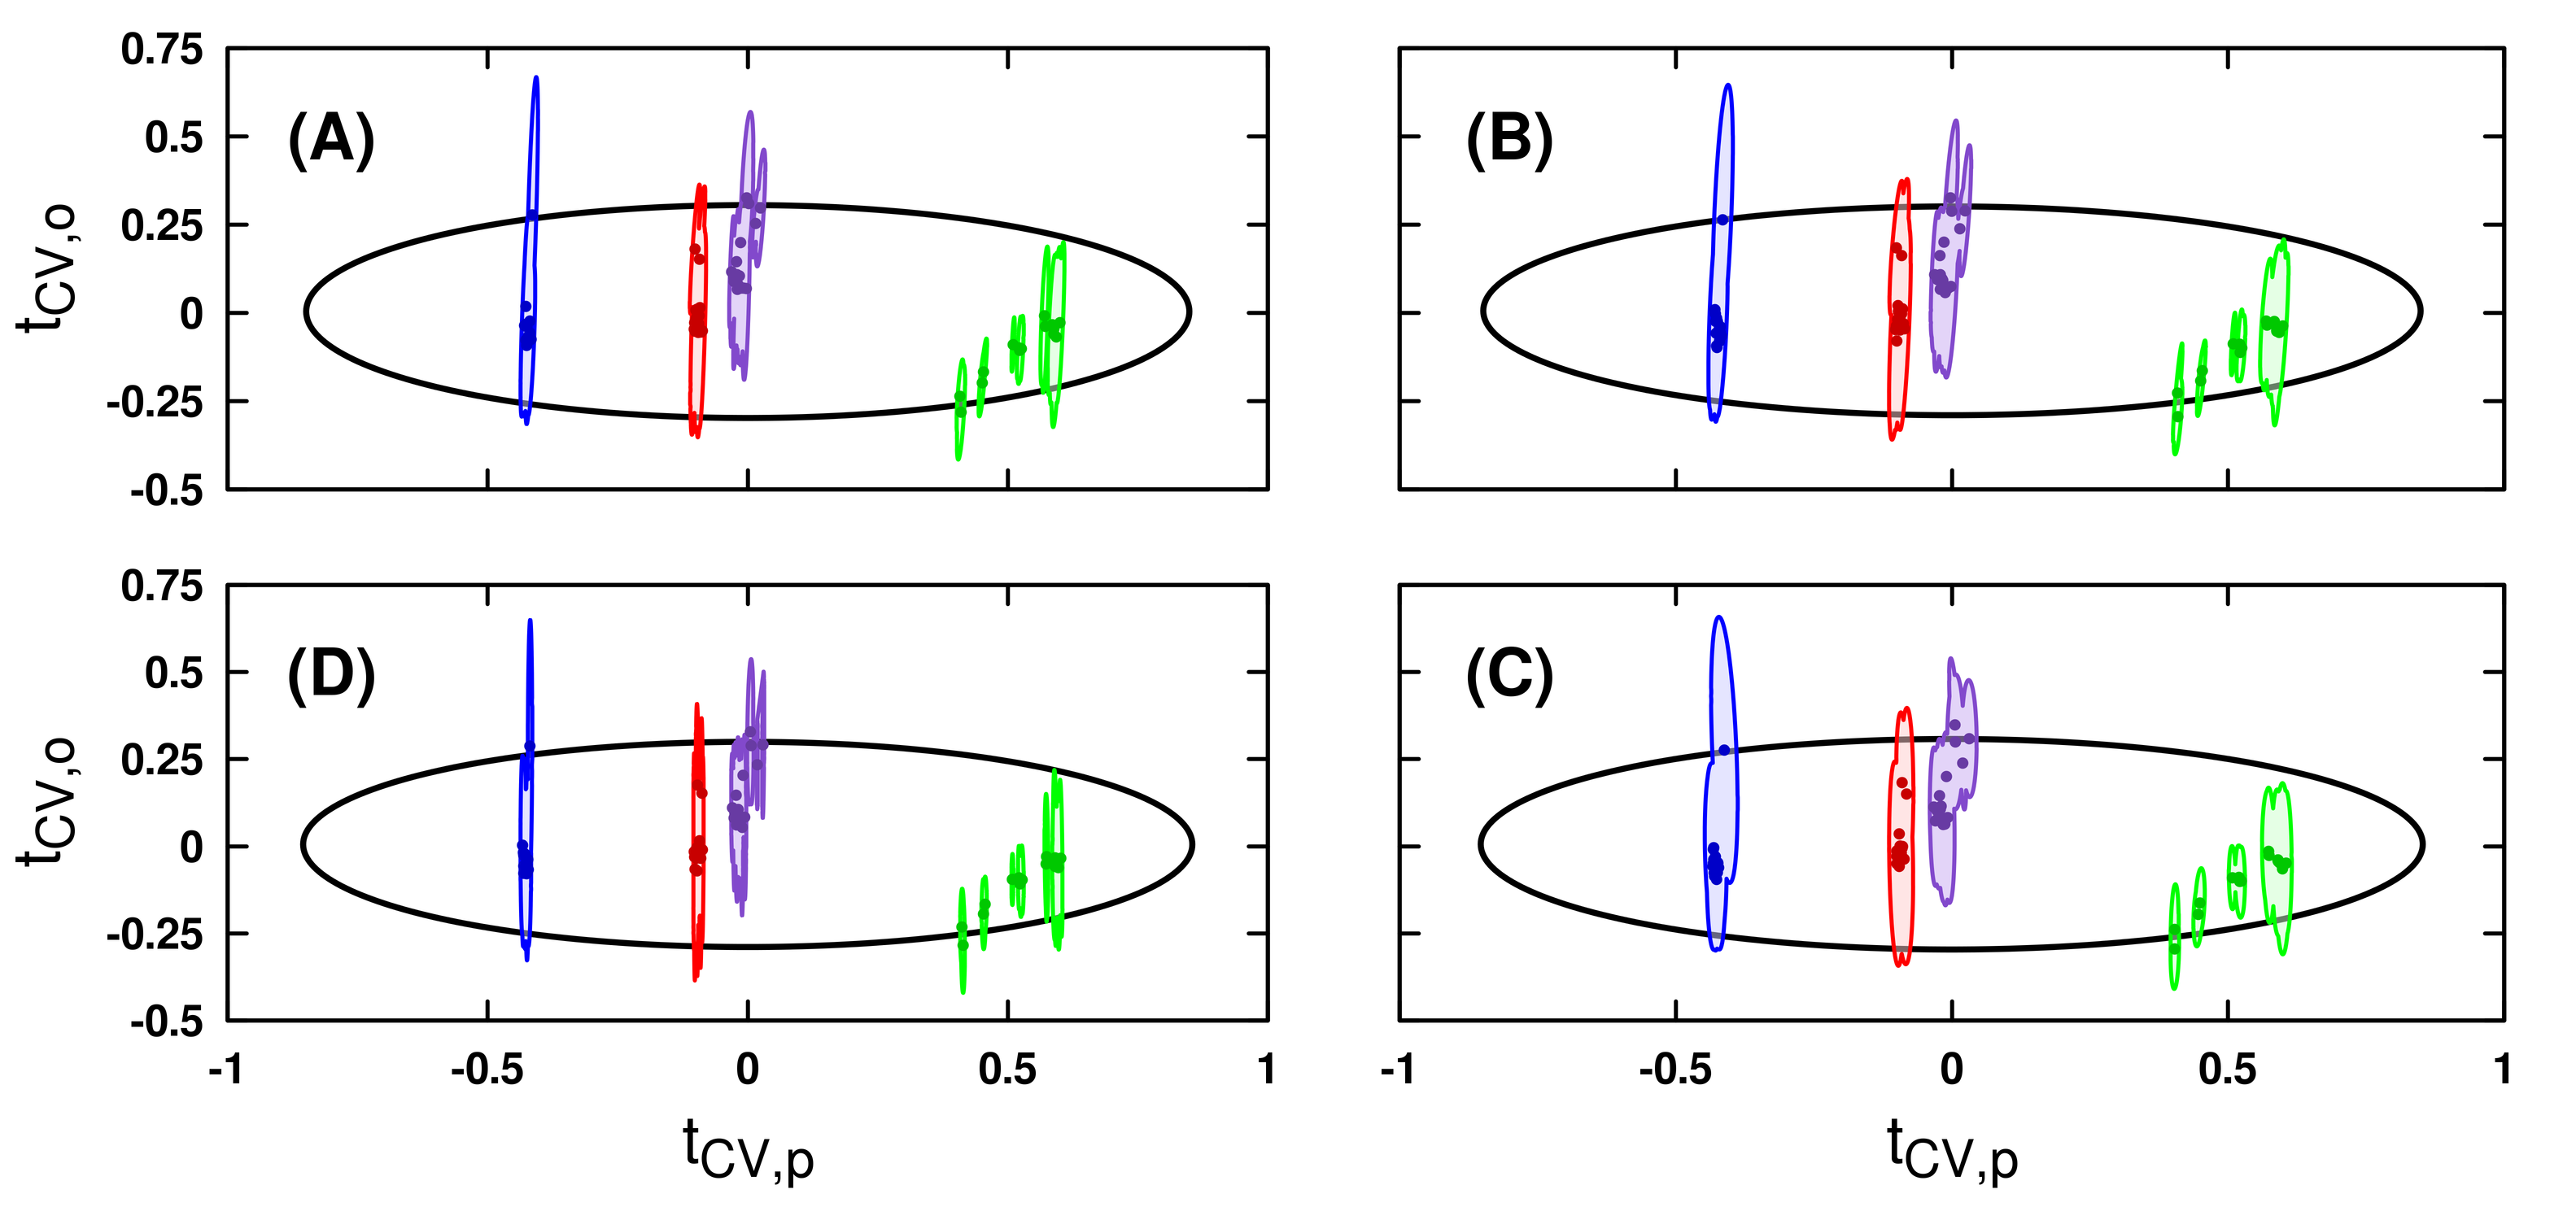
\includegraphics[width=6.5in]{figs/apps/06-oplsr-tcv.png}
\caption
      [Coffees OPLS-R Cross-validated Scores.]{
  {\bf Coffees OPLS-R Cross-validated Scores.}
  \\
  OPLS-R scores of the four coffee roasts, where each roast was regressed
  against its caffeine concentration, as in Figure 4.5. Mean score values
  and confidence ellipses for each observation were computed from 100
  iterations of seven-fold Monte Carlo internal cross-validation.
}
\end{figure}

\begin{doublespace}
Notably, the UV/Vis-estimated caffeine concentration of the dark roast coffee
was slightly higher than that of the medium roast, which is contrary to
expectation given that the coffees were brewed using equal volumes of
grounds. However, OPLS-R of the NMR data using the estimated caffeine
concentrations correctly ranked the roasts according to expectation
(Figure 4.5A). When more orthogonal components were allowed into the OPLS-R
model, the dark roast again shifted to a higher caffeine concentration,
beautifully indicating the presence of overfitting (Figure 4.5B--D).
Monte Carlo cross-validated scores further supported the fact that a $1+1$
OPLS model was the most appropriate (Figure 4.6). Therefore, an OPLS-R model
having only a single orthogonal component was chosen, given the fact that it
more faithfully modeled the underlying NMR data at the expense of
contradicting the more uncertain UV/Vis measurements.
\\\\
Finally, no discernable difference was observed between the 1D \hnmr{} NMR
spectra acquired with and without $T_2$-filtering. Spectra collected on
in-house brewed coffee exhibited high levels of protein background signal,
which were readily suppressed using the CPMG-$z$ pulse sequence element. On
the other hand, the spectra of the four purchased roasts showed no such
background signal, possibly due to more correct brewing technique.
\end{doublespace}

\section{Fingerprinting of Joint \hnmr{} NMR and DI-ESI-MS Data}

\begin{doublespace}
Multiblock bilinear factorizations such as CPCA, MB-PLS and MB-OPLS provide a
powerful framework for analyzing a set of multivariate observations from
multiple analytical measurements containing potentially correlated variables
\cite{westerhuis:jchemo1997,westerhuis:jchemo1998,smilde:jchemo2003}. Such
algorithms provide analogous information to PCA, PLS and OPLS in situations
where extra knowledge is available to subdivide the measured variables into
multiple ``blocks''. As a result, the correlation structures of each block
\emph{and} the between-block correlations may be simultaneously utilized.
Due to the existence of common trends among all blocks, this use of
between-block correlations during modeling will ideally bring the model
loadings (latent variables) into better agreement with the true underlying
biochemistry (hidden variables). In short, multiblock algorithms provide an
ideal means of integrating 1D \hnmr{} NMR and direct injection electrospray
mass spectrometry (DI-ESI-MS) datasets for metabolic fingerprinting
\cite{xu:abc2013}.
\\\\
Consensus PCA (\hyperlink{subsection.3.5.4}{CPCA-W}),
Multiblock PLS (\hyperlink{subsection.3.5.5}{MB-PLS}), and
Multiblock OPLS (\hyperlink{subsection.3.5.6}{MB-OPLS}) were used to analyze
1D \hnmr{} NMR and DI-ESI-MS data collected on metabolite extracts from
human dopaminergic neuroblastoma cells (SK-N-SH) after different neurotoxin
treatments \cite{marshall:metab2015}. Each dataset was also individually
subjected to single-block modeling by PCA and PLS in order to highlight the
information gained by jointly modeling the data within multiblock frameworks.
\end{doublespace}

\subsection{Materials and Methods}

\subsubsection{NMR Acquisition and Processing}

\begin{doublespace}
NMR data were collected and processed according to previously described
procedures \cite{zhang:jiomic2013}. A Bruker Avance DRX 500 MHz spectrometer
equipped with a 5 mm inverse triple-resonance cryoprobe (\hnmr{}, \cnmr{},
\nnmr{}) with a $z$-axis gradient, a BACS-120 sample changer, and an automatic
tuning and matching accessory were utilized for automated NMR data collection.
Free induction decays were collected into 32$k$ complex data points over a
spectral window of $2,342 \pm 2,741$ ppm, using the SOGGY water suppression
pulse sequence (\emph{zgesgp}, \cite{hwang:jmr1995,nguyen:jmr2007}).
\\\\
Following acquisition, the 1D \hnmr{} NMR free induction decays were processed
in the MVAPACK toolbox \cite{worley:acscb2014}. A 1.0 Hz exponential
apodization fuction and a single round of zero-filling were applied prior to
Fourier transformation. Spectra were then automatically phased and normalized
using phase-scatter correction (PSC, \cite{worley:cils2014},
cf. \hyperlink{chapter.6}{Chapter 6}). Finally, chemical shift regions
containing spectral baseline noise or solvent signals were manually removed.
Binning of the processed NMR spectra was performed using the Adaptive
Intelligent (AI) binning algorithm that avoids splitting signals into
multiple bins \cite{demeyer:anchem2008}.
\end{doublespace}

\subsubsection{MS Acquisition and Processing}

\begin{doublespace}
Mass spectra of the SK-N-SH metabolite extracts were acquired in positive ion
mode over a mass range of $m/z$ 50--1,200. Spectra were acquired for 30 s each
using the following source conditions: 2.5 kV electrospray capillary voltage,
60 V sampling cone voltage, 4.0 V extraction voltage, $80^\circ$C source
temperature, $250^\circ$C desolvation temperature, 500 L/h desolvation gas
flow rate, and 15 $\mu$L/min injection flow rate.
\\\\
The initial stages of mass spectral data processing were performed using
MassLynx V4.1 (Waters Corp., Milford, MA). A background subtraction was
performed on all spectra: reference spectra of either paraquat,
1-methyl-4-phenylpyridinium (MPP$^+$), rotenone, or 6-hydroxydopamine (6-OHDA)
in H$_2$O/CH$_3$OH/HCO$_2$H (49.75:49.75:0.5) at 10 ppm were used as
backgrounds. Background subtraction of each spectrum was performed in a
class-dependent manner (e.g. the MPP$^+$ reference mass spectrum was used as
background for MPP$^+$-treated cell samples). As a result, mass spectral
signals from the drugs themselves were guaranteed to not influence subsequent
analyses. The background-subtracted mass spectra were then loaded into MVAPACK
for binning and normalization. All mass spectra were linearly re-interpolated
onto a common axis that spanned from $m/z$ 50--1,200 in 0.003 $m/z$ steps,
resulting in 383,334 variables prior to processing. Based on the low
probability of observing a metabolite in the mass range $m/z$ 1,100--1,200,
the region was removed prior to binning. Mass spectra were uniformly binned
using a bin width of 0.5 $m/z$, resulting in a data matrix of 2,095 variables.
Finally, the MS data matrix observations were normalized using probabilistic
quotient (PQ) normalization \cite{dieterle:anchem2006}.
\end{doublespace}

\subsubsection{Multivariate Statistical Analysis}

\begin{doublespace}
Using functions available in the latest version of MVAPACK, the NMR and MS
data were joined into a single multiblock data structure and modeled using
CPCA-W, MB-PLS and MB-OPLS. Both blocks were scaled to unit variance prior
to modeling, and equal contribution of each block to the models (fairness)
was ensured by further scaling each block by the square root of its variable
count \cite{smilde:jchemo2003}. For the purposes of comparison, PCA and PLS
models of the independent NMR and MS data matrices were also constructed.
All PLS models were trained on a binary discriminant response matrix
(i.e. PLS-DA), in which untreated cells were assigned for one class,
and all neurotoxin-treated cells were assigned to a second class.
\end{doublespace}

\subsubsection{Cross-validation of Multivariate Models}

\begin{doublespace}
Initially, all PCA and CPCA-W models were internally cross-validated using a
leave-one-out (LOOCV) procedure in MVAPACK during model training
\cite{eshghi:cils2014}. A subsequent set of PCA models was trained and
cross-validated using a Monte Carlo seven-fold (MCCV) procedure that
produced less optimistic \qsq{} statistics. All PLS-DA, MB-PLS-DA and
MB-OPLS-DA models were internally cross-validated using a Monte Carlo
seven-fold procedure \cite{wold:cils2001}. All MCCV rounds involved 50
iterations per tested model component. The results of cross-validation
were summarized by per-component \qsq{} statistics, and the number of model
components was chosen such that the cumulative \qsq{} was a strictly increasing
function of component count. Response permutation tests of all supervised
models were performed with 1,000 permutations each to assess the statistical
significance of \rsqy{} and \qsq{} values \cite{westerhuis:metab2008a}.
CV-ANOVA significance tests \cite{eriksson:jchemo2008} were also performed
to supplement the results of the permutation tests.
\end{doublespace}

\begin{SCfigure}
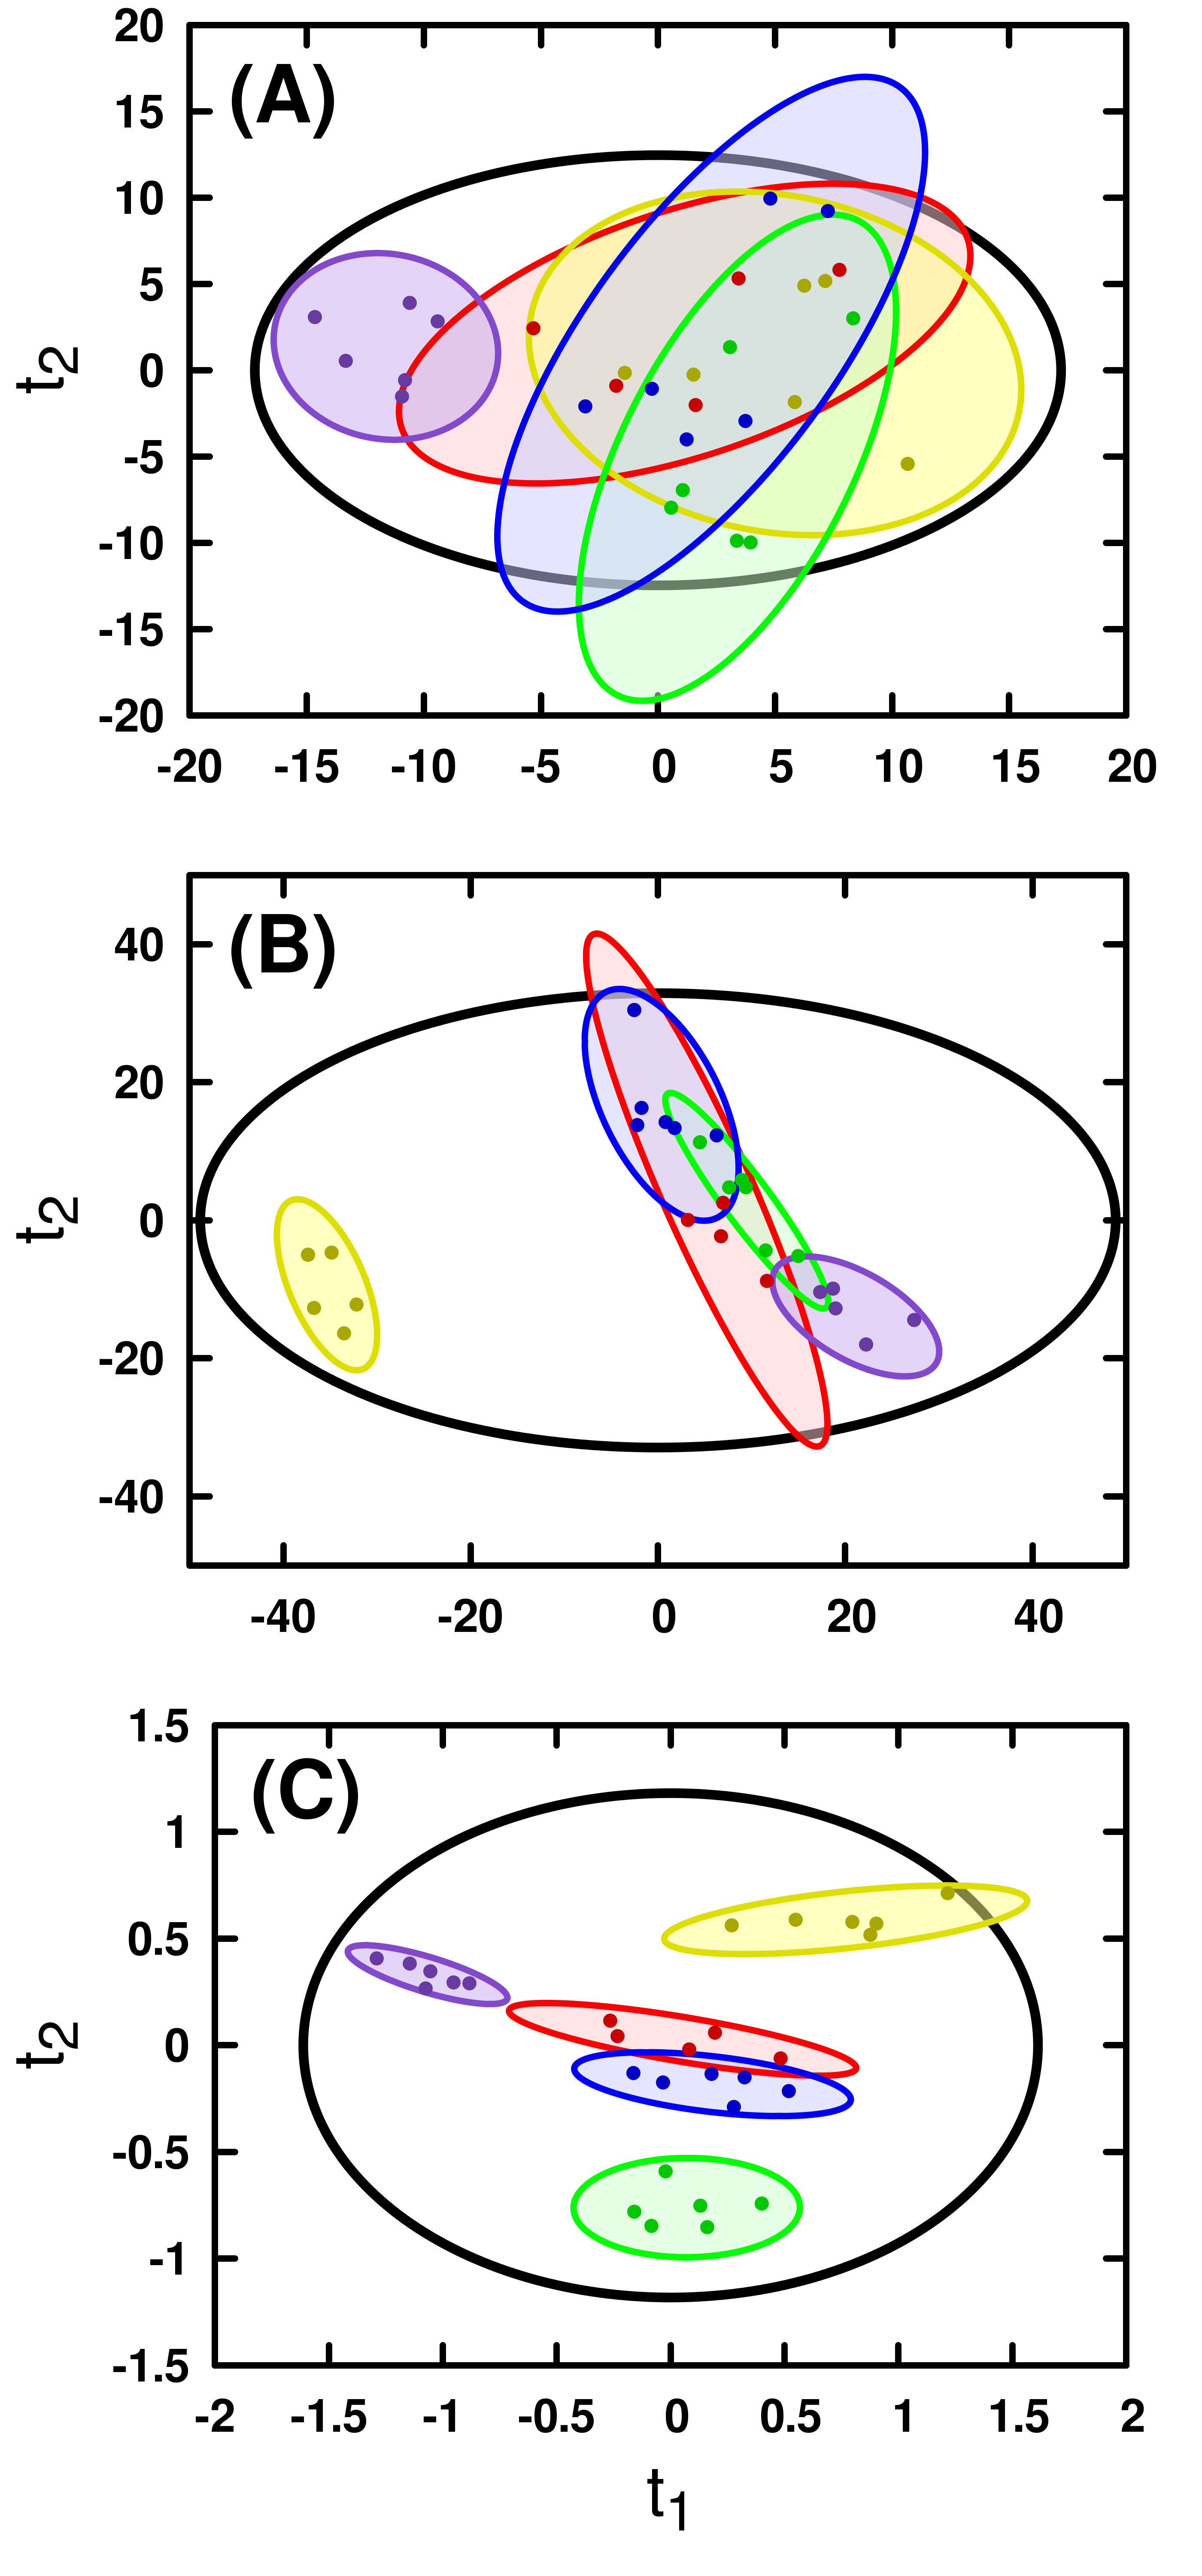
\includegraphics[width=3.5in]{figs/apps/07-mbpca-t.png}
\caption
      [Comparison of PCA and MB-PCA Scores.]{
  {\bf Comparison of PCA and MB-PCA Scores.}
  \\
  Scores generated from ({\bf A}) PCA of \hnmr{} NMR in vacuo, ({\bf B}) PCA
  of DI-ESI-MS in vacuo, and ({\bf C}) MB-PCA of \hnmr{} NMR and DI-ESI-MS.
  Separations between classes are increased upon combination of the two
  data matrices via MB-PCA. Yellow, red, green, violet and blue scores
  correspond to the control, 6-OHDA, MPP$^+$, paraquat and rotenone classes,
  respectively.
}
\end{SCfigure}

\begin{SCfigure}
\includegraphics[width=2.5in]{figs/apps/08-mbpca-d.png}
\caption
      [Dendrograms of PCA and MB-PCA Scores.]{
  {\bf Dendrograms of PCA and MB-PCA Scores.}
  \\
  Dendrograms computed from scores-space class separations
  \cite{worley:abio2013} in the in vacuo PCA and MB-PCA models. Panels
  ({\bf A--C}) correspond to scores in panels ({\bf A--C}) in Figure 4.7,
  above.
}
\end{SCfigure}

\subsection{Results and Discussion}

\subsubsection{Classical Modeling}

\begin{doublespace}
PCA of the binned NMR data matrix ($N = 29, K = 159$) resulted in 10 principal
components having cumulative \rsqx{} and \qsq{} statistics of 0.9485 and
0.4591, respectively, based on LOOCV. Overall, no patterns were readily
discernable in the NMR PCA scores (Figure 4.7A) due to high within-class
variation in the data. However, scores for paraquat treatment were found
to significantly separate from all other classes ($p < 0.002$) along the
first principal component. Scores from PCA of the binned MS data matrix
($N = 29, K = 2,095$) were found to exhibit markedly less within-class
variation compared to the NMR data (Figure 4.7B). Using LOOCV, three
significant components were identified from the binned MS data, yielding
fairly low cumulative \rsqx{} and \qsq{} statistics of 0.3397 and 0.1590.
While paraquat treatment still separated from other drug treatments in MS
PCA scores space, the greatest separations were observed between treated
and untreated (control) cells ($p < 1.0 \times 10^{-9}$). These differing
patterns of separation in NMR and MS PCA scores suggested that multiblock
analyses could provide further information, ideally separating both control
and paraquat scores from all other classes. Figure 4.8 contains dendrograms
of scores-space class separation for each scores plot in Figure 4.7.
\\\\
Per-component \qsq{} statistics computed from LOOCV of the NMR and MS PCA
models suggested fairly marginal model reliability at component counts greater
than one, so follow-up analyses were performed using MCCV on the same data
matrices to obtain less optimistic estimates of reliability. In both cases,
MCCV produced single-component PCA models, indicating that the LOOCV had
substantially over-estimated the number of principal components in each
matrix. A comparison of the resulting \qsq{} statistics from LOOCV and MCCV
is shown in Figure 4.9.
\\\\
PLS-DA of the full-resolution NMR ($N = 29, K = 16,138$) and
MS ($N = 29, K = 2,095$) data matrices both resulted in two-component models.
With the exception of the algorithmically forced separation between control
and treatment classes, similar clustering patterns were observed when compared
to the PCA scores (cf. Figure 4.10A--B). MCCV results from the
NMR ($R^2_Y = 0.9519, Q^2 = 0.7303 \pm 0.0517$) and
MS ($R^2_Y = 0.9951, Q^2 = 0.9440 \pm 0.01142$) PLS-DA models indicated
reasonable levels of response fit and predictive ability. Further validation
by CV-ANOVA \cite{eriksson:jchemo2008} indicated reliable models with $p$
values of 0.002 and $9.8 \times 10^{-6}$ for NMR and MS data, respectively.
Response permutation tests for both PLS-DA models returned $p < 0.001$,
supporting the CV-ANOVA test results.
\end{doublespace}

\begin{SCfigure}
\includegraphics[width=3.5in]{figs/apps/09-rqpca.png}
\caption
      [Comparison of LOOCV and MCCV \qsq{} Statistics for PCA.]{
  {\bf Comparison of LOOCV and MCCV \qsq{} Statistics for PCA.}
  \\
  \rsq{} (red), $Q^2_{\mathrm{LOOCV}}$ (green) and $Q^2_{\mathrm{MCCV}}$ (blue)
  statistics from ({\bf A}) PCA of \hnmr{} NMR in vacuo, ({\bf B}) PCA of
  DI-ESI-MS in vacuo, and ({\bf C}) MB-PCA of \hnmr{} NMR and DI-ESI-MS.
  In all cases, MCCV indicates that both datasets contain a single significant
  principal component, while LOOCV over-estimates the number of significant
  components.
}
\end{SCfigure}

\begin{SCfigure}
\includegraphics[width=3.5in]{figs/apps/10-mbpls-t.png}
\caption
      [Comparison of PLS-DA and MB-PLS-DA Scores.]{
  {\bf Comparison of PLS-DA and MB-PLS-DA Scores.}
  \\
  Cross-validated scores generated from ({\bf A}) PLS-DA of \hnmr{} NMR in
  vacuo, ({\bf B}) PLS-DA of DI-ESI-MS in vacuo, and ({\bf C}) MB-PLS-DA of
  \hnmr{} NMR and DI-ESI-MS. Consensus directions in MB-PLS-DA scores space
  show decreased rotation during cross-validation when compared to PLS-DA
  scores of the in vacuo PCA model. Yellow, red, green, violet and blue scores
  correspond to the control, 6-OHDA, MPP$^+$, paraquat and rotenone classes,
  respectively.
}
\end{SCfigure}

\subsubsection{Multiblock Modeling}

\begin{doublespace}
Identification of consensus directions in the NMR and MS data matrices that
maximally captured overall variation (MB-PCA) or response correlations (MB-PLS)
resulted in more informative models than those calculated against either NMR
or MS in vacuo. Using MB-PCA with LOOCV, five significant components were
identified ($Q^2 = 0.2322$) that cumulatively explained comparable amounts
of variation in the NMR ($R^2_X = 0.8528$) and MS ($R^2_X = 0.5015$) blocks
relative to the individual PCA models. As expected, MB-PCA combined the
information from both blocks to dramatically increase class separations in
super-scores space (Figure 4.7C). More specifically, both control and paraquat
classes were separated from other neurotoxin treatments, predominantly along
the first principal component. Furthermore, MPP$^+$ treatment exhibited
significant separation from 6-OHDA and rotenone treatments, which was not
expected from examination of the individual NMR or MS PCA scores.
\end{doublespace}

\begin{figure}[ht!]
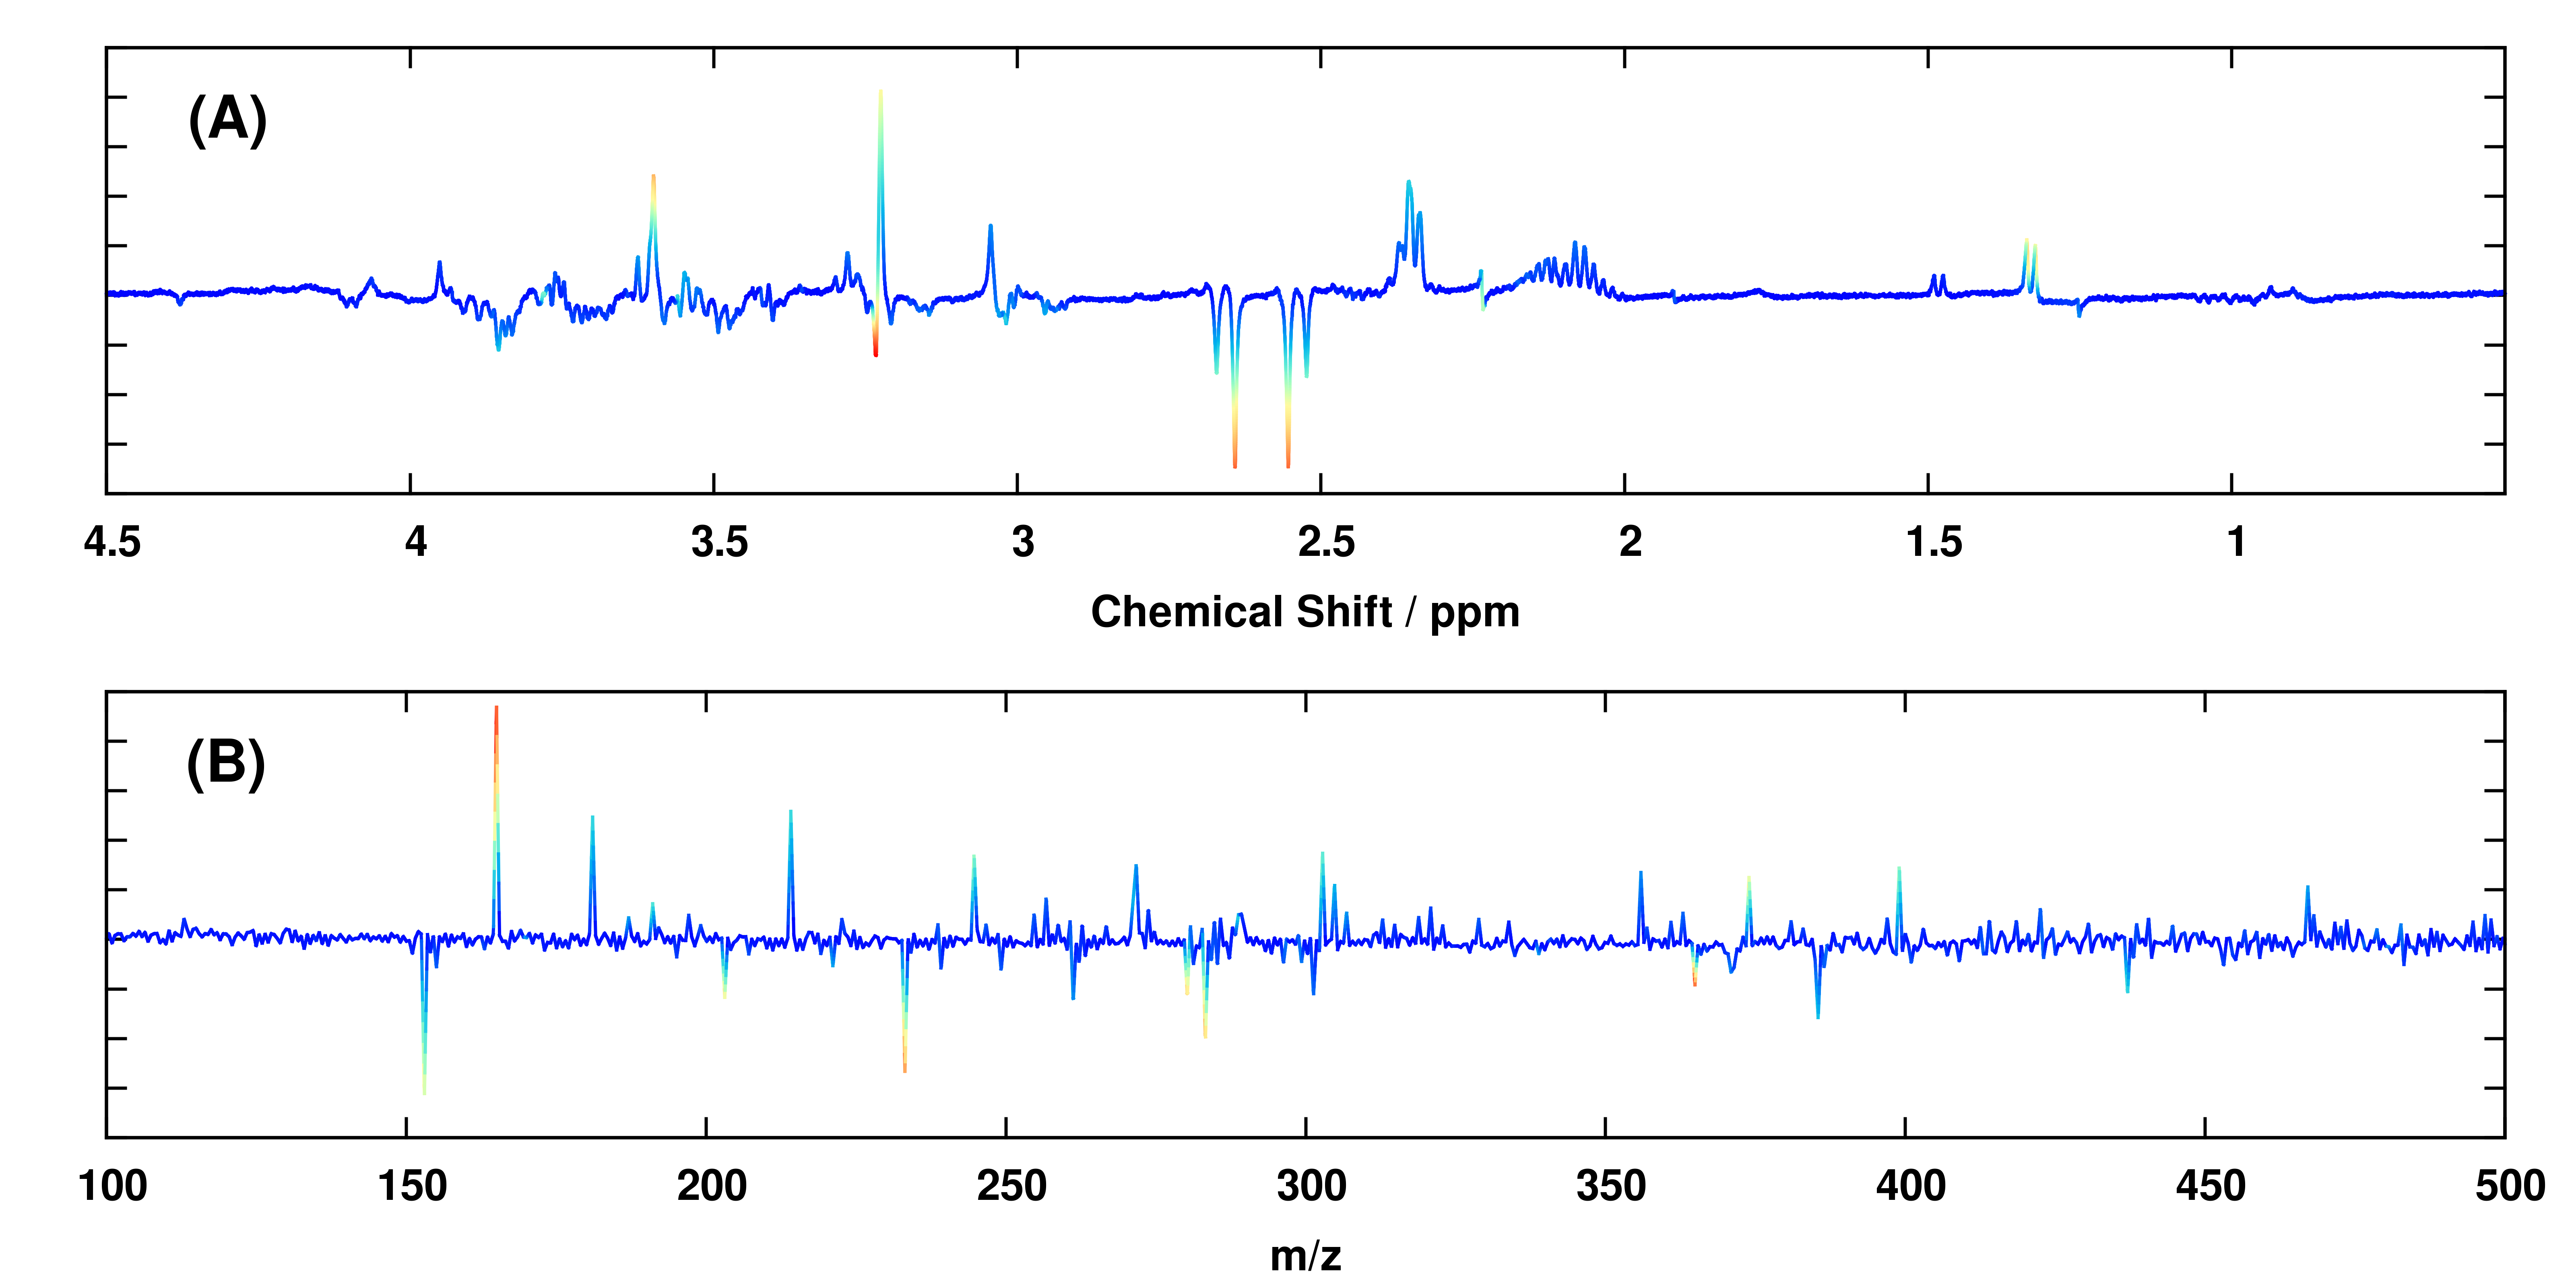
\includegraphics[width=6.5in]{figs/apps/11-mbpls-p.png}
\caption
      [Backscaled NMR and MS Block Loadings.]{
  {\bf Backscaled NMR and MS Block Loadings.}
  \\
  Backscaled ({\bf A}) \hnmr{} NMR block and ({\bf B}) DI-ESI-MS block loadings
  from MB-PLS-DA. Comparison of the above panels to those from MB-OPLS-DA
  (Figures 4.12, 4.13) reveals the mixed predictive and orthogonal variation
  present in MB-PLS loadings. It is also important to note that a second
  PLS component exists, and thus complete interpretation of the joint NMR
  and MS data requires simultaneous examination of \emph{two} sets of
  block loadings.
}
\end{figure}

\begin{doublespace}
Subsequent re-evaluation of the MB-PCA model's reliability using MCCV reduced
the number of expected significant components to two (Figure 4.9C). However,
secondary and higher components' \qsq{} statistics were still found to be
statistically indistinguishable from zero, which further suggests that only
one principal direction exists in the binned NMR and MS data matrices that
captures any substantial variation.
\end{doublespace}

\begin{figure}[ht!]
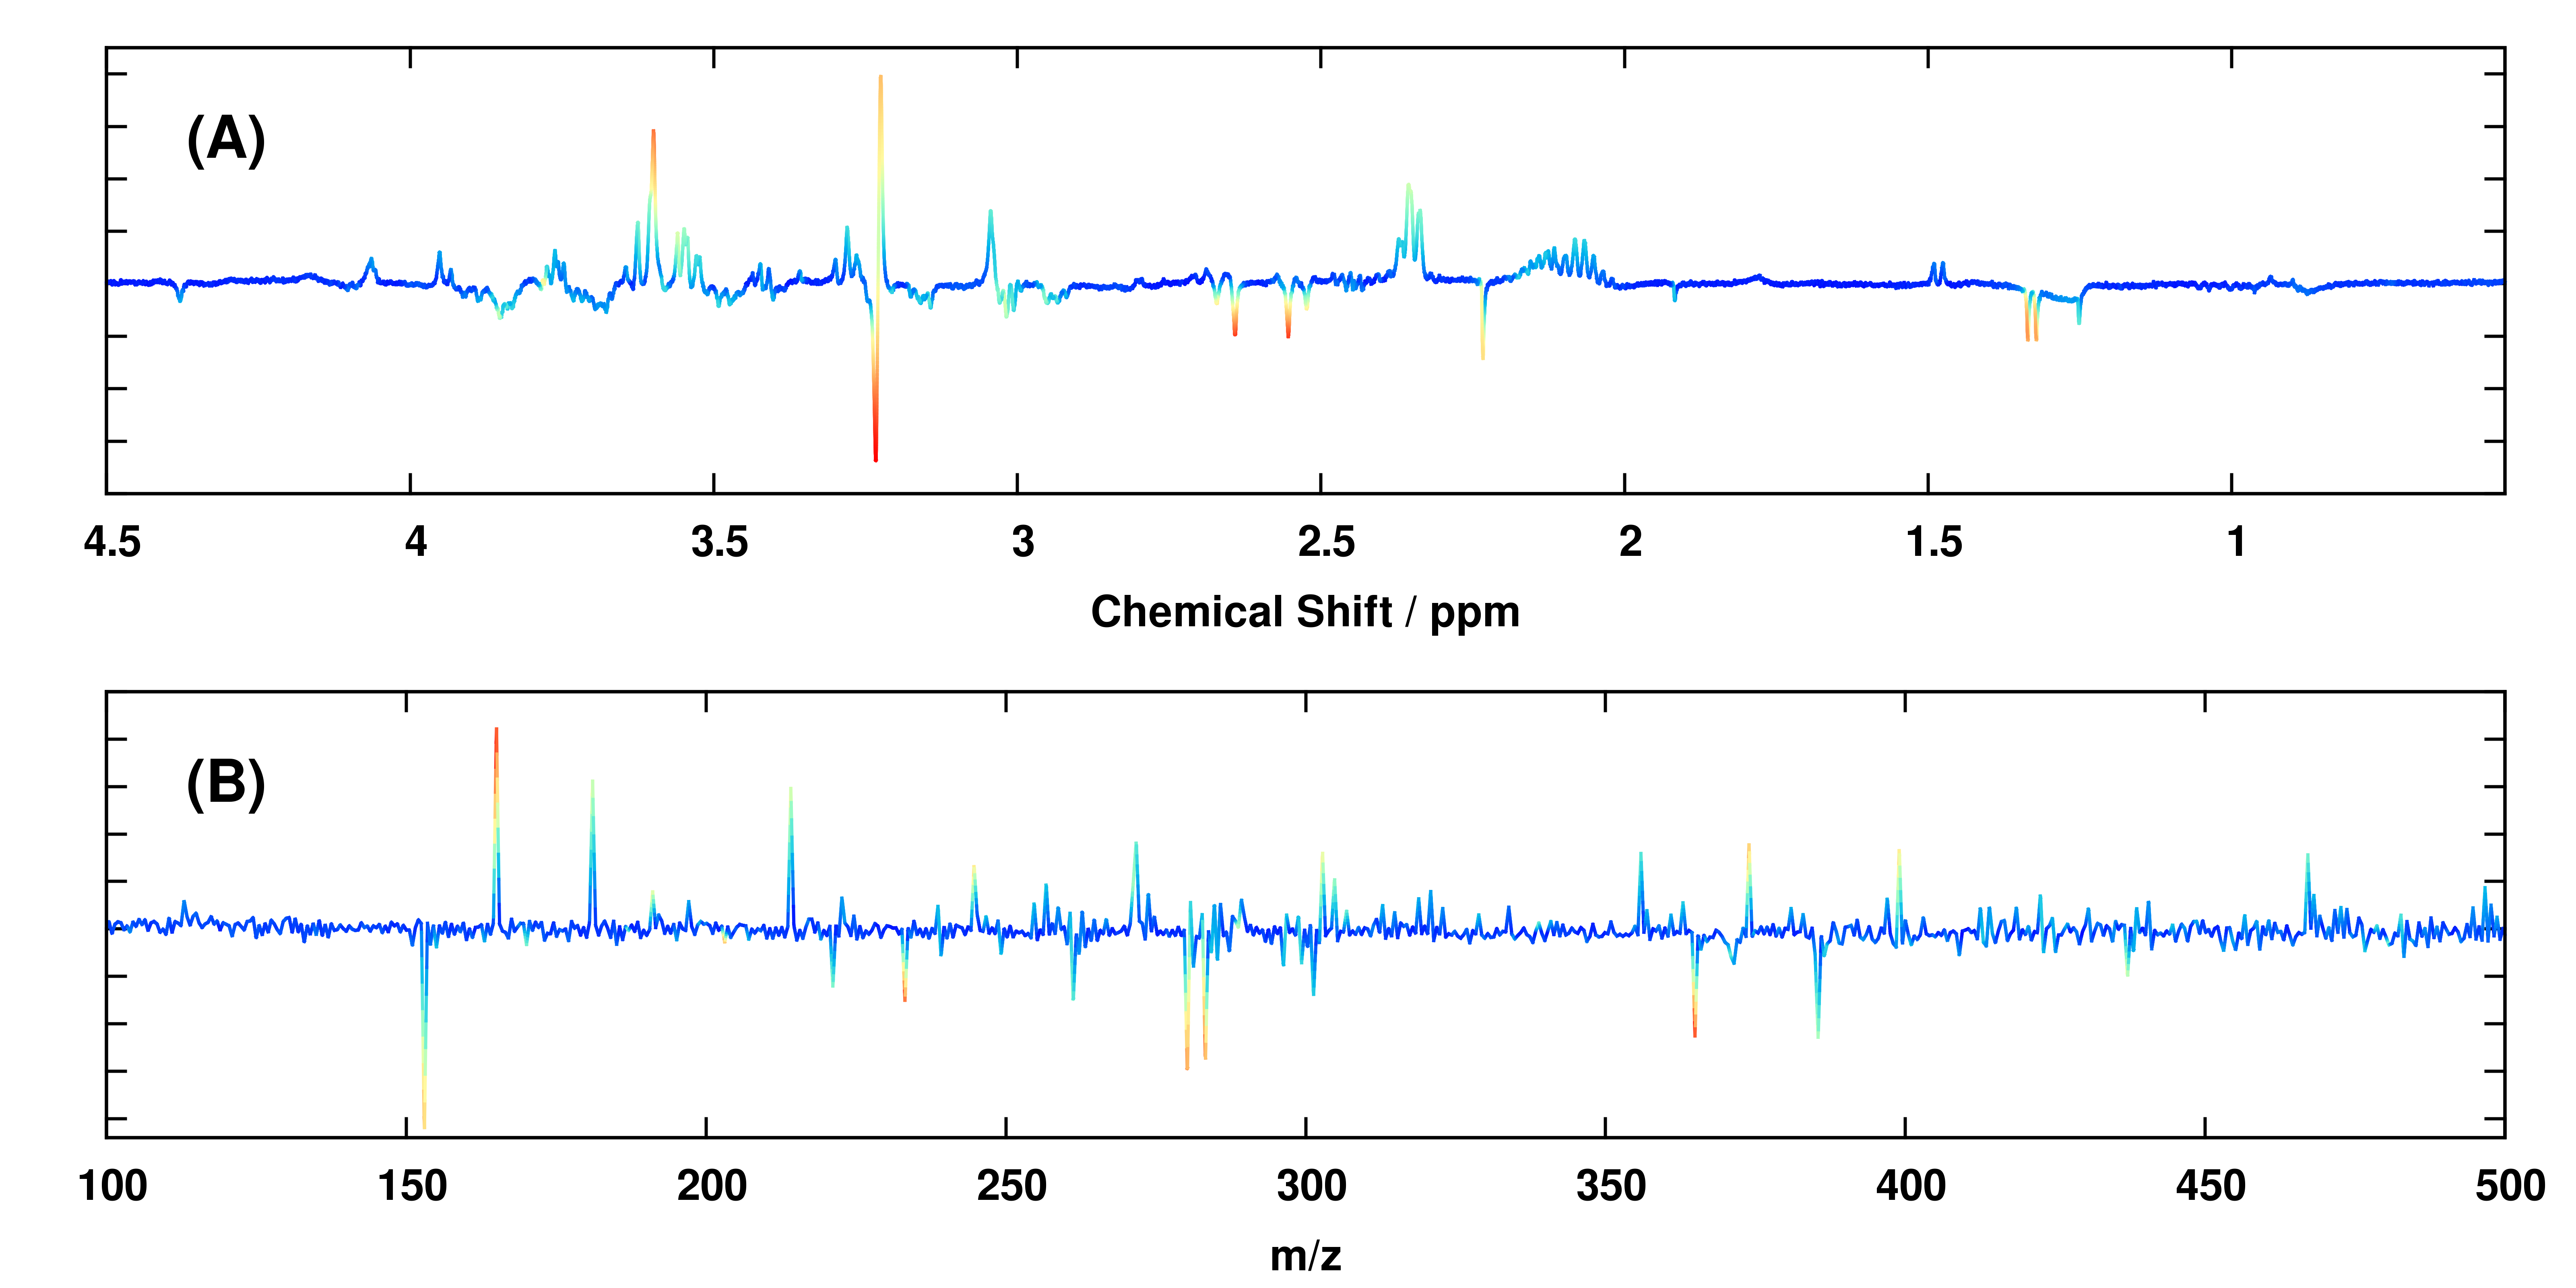
\includegraphics[width=6.5in]{figs/apps/12-mbopls-p.png}
\caption
      [Backscaled NMR and MS Predictive Block Loadings.]{
  {\bf Backscaled NMR and MS Predictive Block Loadings.}
  \\
  Backscaled predictive ({\bf A}) \hnmr{} NMR block and ({\bf B}) DI-ESI-MS
  block loadings from MB-OPLS-DA.
}
\end{figure}

\begin{figure}[ht!]
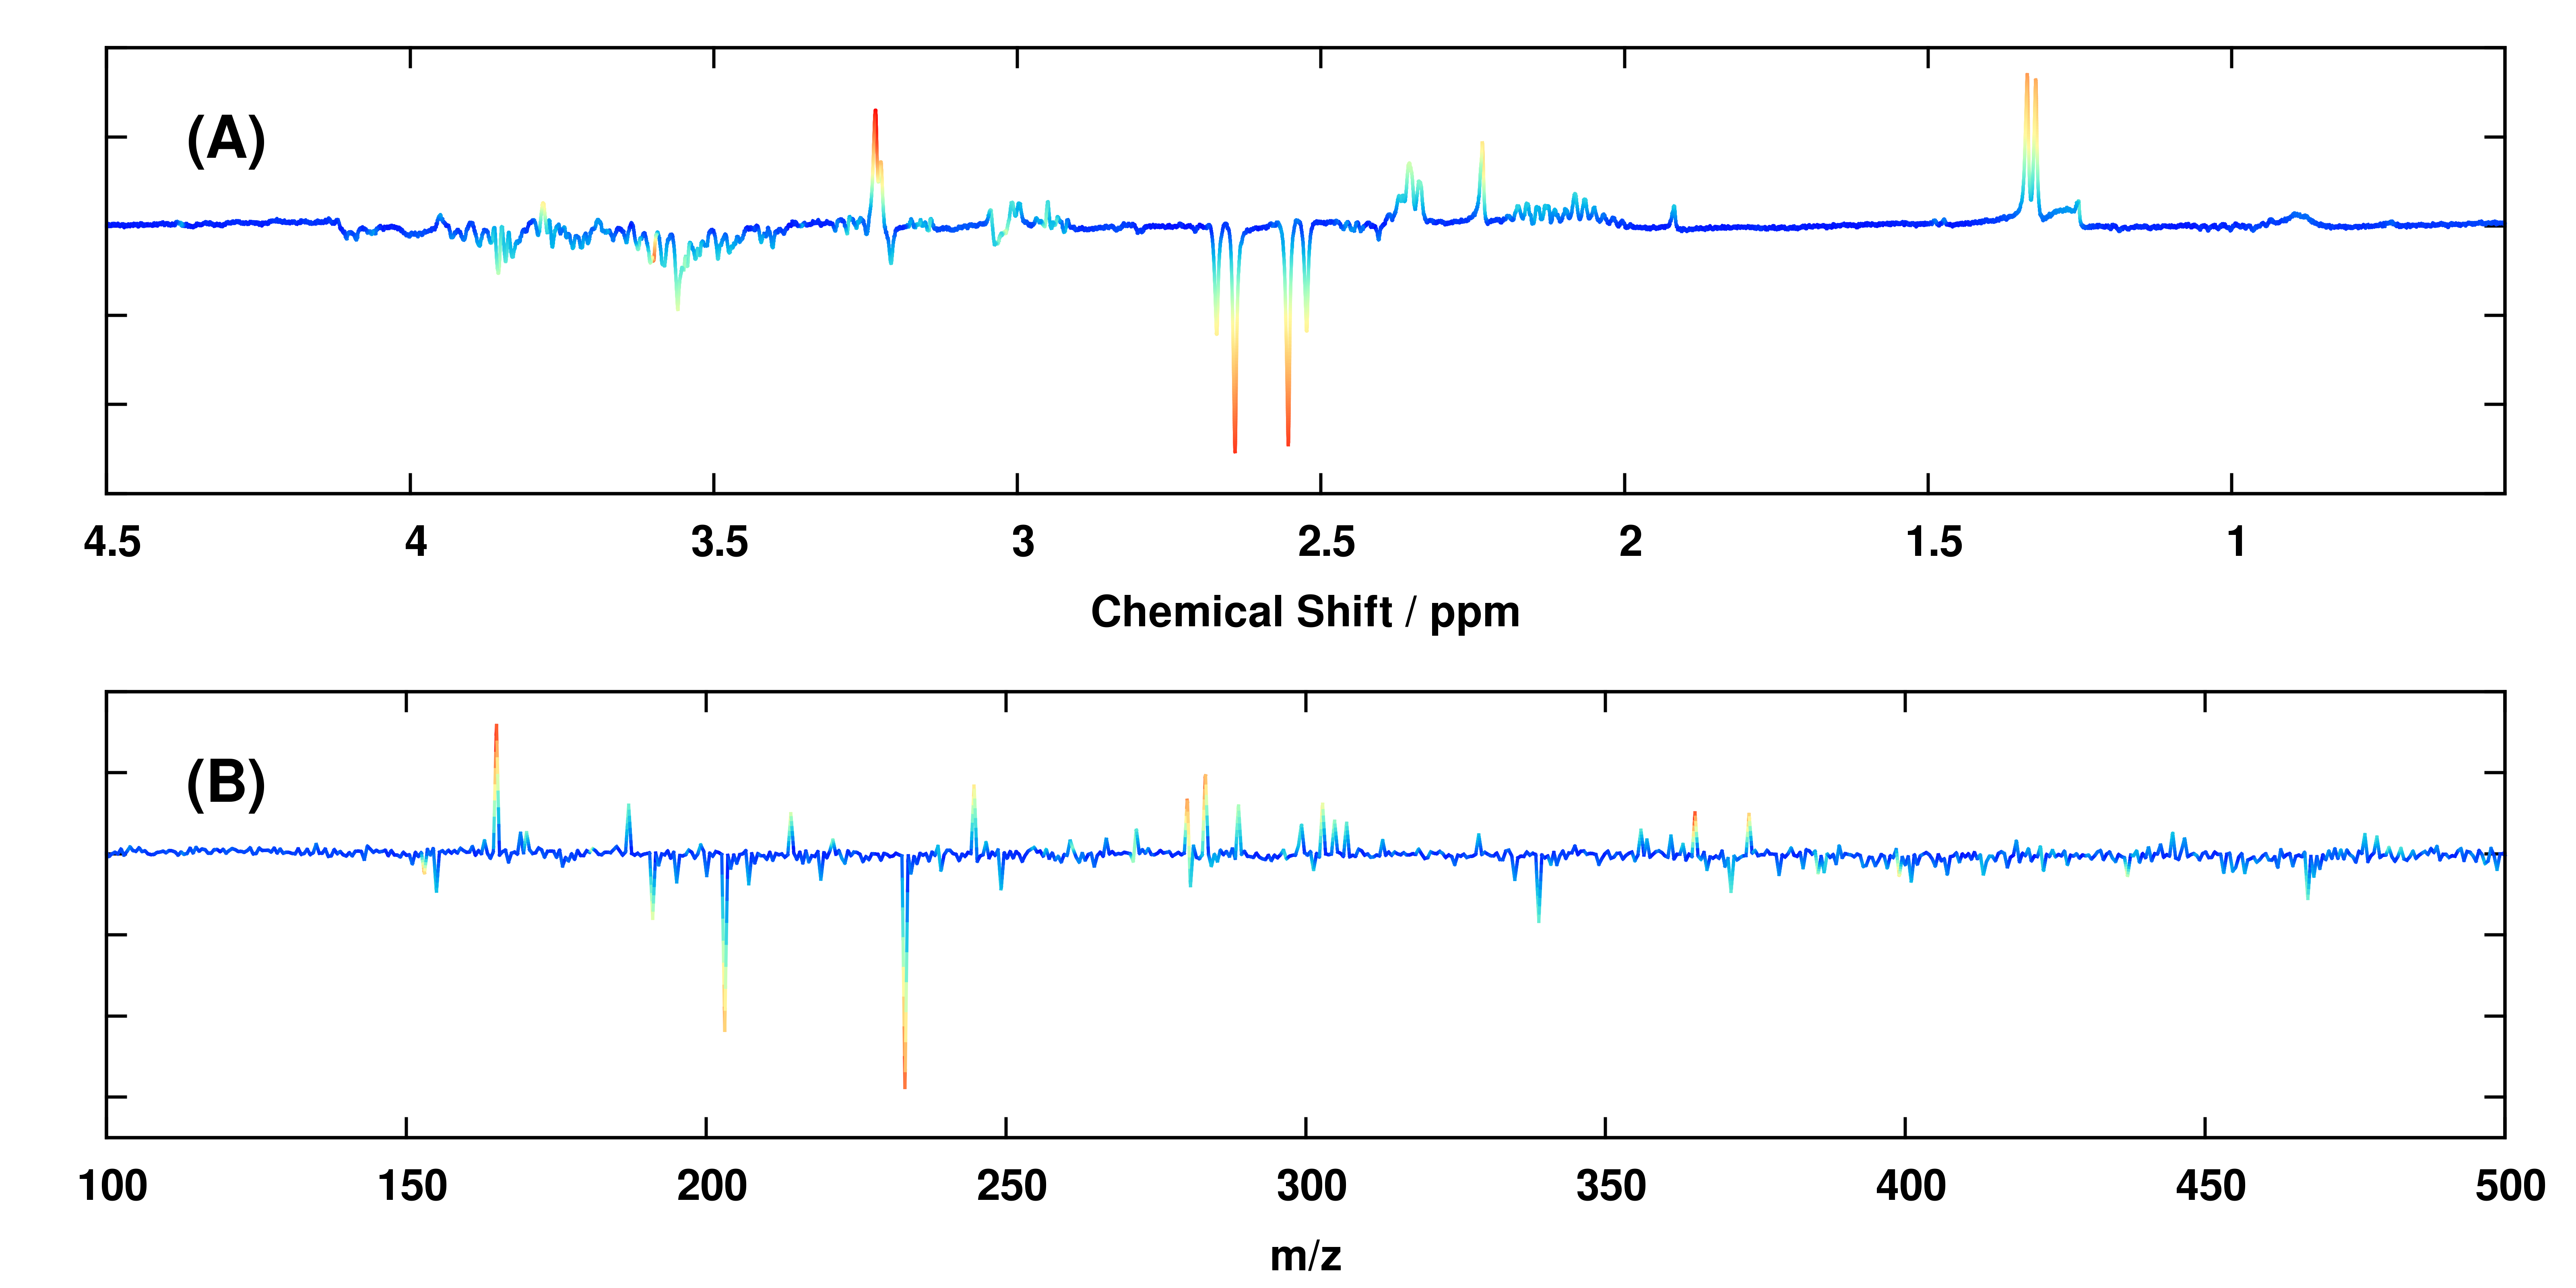
\includegraphics[width=6.5in]{figs/apps/13-mbopls-po.png}
\caption
      [Backscaled NMR and MS Orthogonal Block Loadings.]{
  {\bf Backscaled NMR and MS Orthogonal Block Loadings.}
  \\
  Backscaled orthogonal ({\bf A}) \hnmr{} NMR block and ({\bf B}) DI-ESI-MS
  block loadings from MB-OPLS-DA.
}
\end{figure}

\begin{doublespace}
MB-PLS of the data yielded similar improvements in model information content.
Two significant components were identified
($R^2_Y = 0.9876, Q^2 = 0.9014 \pm 0.0185$) that clearly separated control and
paraquat treatment classes from all other classes in scores space
(Figure 4.10). CV-ANOVA testing produced a $p$ value of $3.4 \times 10^{-4}$
and response permutation testing yielded $p < 0.001$, indicating a reliable
MB-PLS-DA model. Backscaled first-component MB-PLS-DA loadings are shown in
Figure 4.11. Modeling the multiblock data with MB-OPLS and MCCV produced a
single predictive component and a single orthogonal component
($R^2_Y = 0.9031, Q^2 = 0.7084 \pm 0.0241$), making later interpretation
markedly simpler (cf. Figures 4.12 and 4.13). Examination of cross-validated
MB-OPLS-DA scores (Figure 4.14) provides an excellent example of how PLS mixes
predictive and compensatory variation. In MB-OPLS super-scores, paraquat
treatment is distinctly separated from other neurotoxin treatment classes along
the orthogonal component ($\mathbf{t_o}$). In the MB-PLS model, this
distinction between paraquat and other drug treatments becomes mixed with the
variation that separates the control class from all drug treatments. In effect,
the two effects have been disentagled in the MB-OPLS model, providing richer
information about the differing mechanisms of each neurotoxic drug. Additional
orthogonal components would serve to further disentangle the two effects, at
the slight expense of model reliability. Validation of the MB-OPLS model by
CV-ANOVA resulted in a $p$ value equal to $5.5 \times 10^{-6}$, and permutation
testing corroborated CV-ANOVA with $p < 0.001$, once again indicating a
reliable supervised model.
\end{doublespace}

\begin{SCfigure}
\includegraphics[width=3.5in]{figs/apps/14-mbopls-t.png}
\caption
      [MB-OPLS-DA Cross-validated Scores.]{
  {\bf MB-OPLS-DA Cross-validated Scores.}
  \\
  Cross-validated scores generated from MB-OPLS-DA of the joint \hnmr{} NMR
  and DI-ESI-MS data. The OPLS filter within MB-OPLS has effectively rotated
  the super-scores of the MB-PLS model (Figure 4.10C) to better differentiate
  between class-predictive and class-orthogonal variation.
}
\end{SCfigure}

\subsection{Conclusions}

\begin{doublespace}
The use of multiblock bilinear factorizations that capitalize on the
availability of blocking information afforded greater model interpretability
with the NMR and MS data than what was provided by single-block methods. The
neurotoxins dataset provided an opportunity to compare the results of LOOCV
and MCCV for optimal principal component count determination when marginally
predictive data is being modeled. As expected, MCCV was a less optimistic
estimator of model reliability than LOOCV, and produced more parsimonious PCA
decompositions. Finally, the dataset was an ideal proving ground for the new
MB-OPLS algorithm, as MB-PLS-DA had clearly mixed class-predictive variation
into multiple components. The use of MB-OPLS-DA resulted in more easily
interpretable backscaled loadings, and provided more information relating to
separations between control and drug treatment \emph{and} separations between
paraquat and other drug treatments (Figure 4.13).
\end{doublespace}

\section{Monte Carlo Analysis of Scores-space Separations}

\begin{doublespace}
FIXME \cite{worley:anchem2015}.
\end{doublespace}

\subsection{Materials and Methods}

\begin{doublespace}
FIXME.
\end{doublespace}

\subsubsection{Initial Datasets}

\begin{doublespace}
FIXME.
\end{doublespace}

\subsubsection{Monte Carlo Simulation}

\begin{doublespace}
FIXME.
\end{doublespace}

\subsection{Results and Discussion}

\begin{doublespace}
FIXME.
\end{doublespace}

\section{Conclusions}

\begin{doublespace}
FIXME.
\end{doublespace}

\bibliographystyle{abbrv}
\bibliography{bworley}

